\chapter{Stochastic switching linear control using linear hybrid models}
\label{sec_rbpf_control}
In Chapter \ref{sec_switch_mpc_lit} model switching MPC was introduced. In short, a set of models with corresponding binary integer variables are incorporated into the MPC optimisation problem. The optimisation algorithm changes the model it uses for prediction based on the location of the previous predicted state. In this way a number of models can potentially be used for prediction. It is desirable to change models if the system states move far away from the linearisation point of current linear model. It is hoped that the significant computational burden this introduces is offset by the increased predictive accuracy of the controller.

In Chapter \ref{sec_linear_control} we developed efficient stochastic controller algorithms (LQG and MPC) which use a single linear model for control. While it is possible to attempt to extend these algorithms to the aforementioned approach, the computational problems will persist because mixed integer programming is fundamentally more difficult than quadratic programming \cite{forst}. From a practical perspective one would like to reduce computational complexity because, especially for large problems, on-line optimisation can become problematic.

In Chapter \ref{sec_inf_lin_hybrid} the Rao-Blackwellised particle filter was introduced. Briefly, the filter uses a set of linear models, $M_i=(A_i, B_i)$ for each model $i$, to estimate the current state (we assume the system and measurement noise is common across all models as well as the observation matrix). The ability of each model to explain the observations is calculated in a Bayesian sense. This is used to weight the importance of each model's contribution to the current state estimate. 

In this chapter we will attempt to combine the ideas of Chapter \ref{sec_switch_mpc_lit}, \ref{sec_linear_control} and \ref{sec_inf_lin_hybrid} to create a computationally efficient switching model controller algorithm. We assume that the underlying process dynamics are described by (\ref{eq_lin_system_in_rbpf}) where $f$ and $g$ are the nonlinear transition and observation functions of the CSTR process introduced in Chapter \ref{sec_cstr}. It is assumed that $x_t$ is a latent stochastic variable and $y_t$ is an observed stochastic variable.
\begin{equation}
\begin{aligned}
x_{t+1} &= f(x_t, u_t) + w_{t+1}  \\
y_{t+1} &= g(x_{t+1}) + v_{t+1}  
\end{aligned}
\label{eq_lin_system_in_rbpf}
\end{equation}
We also assume that the models used for inference and control are linear and of the form shown in (\ref{eq_lin_system_control_rbpf}) for model $M_i=(A_i, B_i)$. 
\begin{equation}
\begin{aligned}
x_{t+1} &= A_ix_t + B_iu_t + w_{t+1} \\
y_{t+1} &= Cx_{t+1} + v_{t+1} 
\end{aligned}
\label{eq_lin_system_control_rbpf}
\end{equation}
The noise terms retain their meaning from Chapter \ref{sec_linear_control}. It is our aim to move the system states from the  unstable (nominal) operating point to another operating point. This will clearly cause the system to traverse the state space and necessitate model switching. We first describe the intuition behind the proposed switching controller algorithm and then state the algorithm.

As mentioned before, it becomes desirable to have a mechanism to switch the underlying controller model if the system states move far away from the linearisation point of the current model. However, it is computationally difficult to perform this switching within the framework of the optimisation algorithm because it invariably necessitates the introduction of integer variables. We propose an algorithm which uses the Rao-Blackwellised particle filter to estimate the current state as well as the models which best describe the current observation. Based on the results of Chapter \ref{sec_inf_lin_hybrid} we expect the weight assigned to each model to skew in favour of the models which were linearised closest to the current state. Now we have two options to implement control at each time step\footnote{Note that $A^*$ is the model used for control in this explanation.}:
\begin{enumerate}
\item
Use only the most likely model (the model with the highest switch weight) for controller prediction i.e. use $A^* = A_{\text{indmax}[s_t]}$.
\item
Use the weighted average (from the switch weight) of the models for controller prediction i.e. use $A^* = \sum_{i=1}^M s_t^i A_i$.
\end{enumerate}
Since it is not clear which approach is best we investigate both. This ``best current model" is then used in the single model controller algorithms discussed in Chapter \ref{sec_linear_control}. This approach falls squarely between the purely single model controllers, as discussed in Chapter \ref{sec_linear_control}, and the switching model controllers, where the model switching occurs inside the optimisation problem, as discussed in Chapter \ref{sec_switch_mpc_lit}. By switching models outside the optimisation problem the scheme will necessarily be more computationally efficient than those found in Chapter \ref{sec_switch_mpc_lit}. 

\textbf{Switching controller algorithm}:
\begin{enumerate}
\item
Use a switching filter algorithm, e.g. the Rao-Blackwellised particle filter, to update the state estimates of the particle population given the current observation. See Chapter \ref{sec_inf_lin_hybrid} for more details.
\item
Select the best current model to for control based on the model weights also supplied by the switching filter algorithm.
\item
Use the mean and covariance information from the current posterior state estimate and the best current model (from step 2) within the context of the stochastic controller (LQG or MPC) formulation of Chapter \ref{sec_linear_control}.
\item
Repeat for the next observation. 
\end{enumerate} 
The astute reader will notice that we are implicitly using the graphical model shown in Figure \ref{fig_gm_filter} for state estimation (filtering) but the graphical model of Figure \ref{fig_gm_prediction} for model based prediction in step 3.
\begin{figure}[H] 
\centering
\begin{tikzpicture}

  % Define nodes
  \node[obs] (ya) {$y_{0}$};
  \node[obs, right=of ya] (yb) {${\hdots}$};
  \node[obs, right=of yb] (yc) {$y_{t}$};
  \node[latent, above=of ya]  (xa) {$x_{0}$};
  \node[latent, above=of yb, right=of xa]  (xb) {${\hdots}$};
  \node[latent, above=of yc, right=of xb]  (xc) {$x_{t}$};
  \node[det, above=of xa, xshift=0.7cm] (da) {$u_{0}$};
  \node[det, above=of xb, xshift=0.7cm] (db) {$u_{t-1}$};
  \node[latent, above=of xa, yshift=1.1cm] (sa) {$s_{0}$};
  \node[latent, above=of xb, yshift=1.1cm] (sb) {${\hdots}$};
  \node[latent, above=of xc, yshift=1.1cm] (sc) {$s_{t}$};
  
  % Connect the nodes
  \edge {da} {xb};
  \edge {db} {xc};
  \edge {xa} {ya};
  \edge {xb} {yb};
  \edge {xc} {yc};
  \edge {xa} {xb};
  \edge {xb} {xc};
  \edge {sa} {sb};
  \edge {sb} {sc};
  \edge {sa} {xa};
  \edge {sb} {xb};
  \edge {sc} {xc};
  
\end{tikzpicture}
\caption{Graphical model used for state estimation.}
\label{fig_gm_filter}
\end{figure}
\begin{figure}[H] 
\centering
\begin{tikzpicture}

  % Define nodes
  \node[obs] (ya) {$y_0$};
  \node[latent, above=of ya]  (xa) {$x_0$};
  \node[latent, above=of yb, right=of xa]  (xb) {$x_1$};
  \node[latent, above=of yc, right=of xb]  (xc) {$x_2$};
  \node[det, above=of xa, xshift=0.7cm] (da) {$u_0$};
  \node[det, above=of xb, xshift=0.7cm] (db) {$u_1$};
  \node[latent, above=of xa, yshift=1.1cm] (sa) {$s_0$};
  
  % Connect the nodes
  \edge {da} {xb};
  \edge {db} {xc};
  \edge {xa} {ya};
  \edge {xa} {xb};
  \edge {xb} {xc};
  \edge {sa} {xa};
\end{tikzpicture}
\caption{Simplified graphical model used for prediction. Within the context of prediction we have that $x_0 \leftarrow x_t$ and $s_0 \leftarrow s_t$ at each successive time step to simplify notation.}
\label{fig_gm_prediction}
\end{figure}
We are not using the graphical model associated with Rao-Blackwellised particle prediction (see Chapter \ref{sec_inf_rbpf_pred}) because that would require that we incorporate stochastic model switching within the optimisation algorithm. 

For the remainder of this chapter we assume that we have a bank of $M$ linear models and that we measure both states. Each model is derived by linearising the non-linear CSTR model, found in Chapter \ref{sec_cstr}, around the nominal operating points discussed in the same chapter as well as Chapter \ref{sec_rbpf_filtering_cstr}. We also use the switching transition matrices $P_2, P_3$ found in (\ref{eq_switch_trans}) where appropriate. All other parameters are the same as those found in Chapter \ref{sec_linear_control}.
\section{Unconstrained switching control}
As mentioned earlier, we will investigate two approaches which can be used to implement the switching controller algorithm. The first approach, used in Chapter \ref{sec_rbpf_control_uncon}, makes use of only the most likely model within the controller. The second approach, discussed in Chapter \ref{sec_ma_rbpf}, makes use of model averaging to construct a model for control.  
\subsection{Most likely model approach}
\label{sec_rbpf_control_uncon}
Due to the analysis of Chapter \ref{sec_uncon_lin_control} we know that it is possible to convert the stochastic optimisation problem (\ref{eq_rbpf_lqg}) into the deterministic optimisation problem (\ref{eq_rbpf_lqr}) for each linear model $(M_1, M_2, M_3)$ given that we have the current state estimate $x_0$, the model dynamics are linear and the underlying distributions are Gaussian. Throughout this chapter we make these assumptions\footnote{Note that the underlying model is clearly nonlinear but the model used for prediction and inference is linear.}. As before, we also denote the mean and covariance of the current state estimate $x_0$ by $\mathbb{E}[x_0]=\mu_0$ and $\text{var}[x_0]=\Sigma_0$. We use a prediction horizon of $N=150$ i.e. 15 minutes into the future.
\begin{equation}
\begin{aligned}
&\underset{\mathbf{u}}{\text{min }} \mathbb{E}\left[ \frac{1}{2}\sum_{k=0}^{N-1} \left( x_k^TQx_k + u_k^TRu_k \right) + \frac{1}{2}x_N^TP_fx_N \right] \\
& \text{subject to } x_{t+1}=A_ix_t+B_iu_t + w_t\\
\end{aligned}
\label{eq_rbpf_lqg}
\end{equation}
We have that (\ref{eq_rbpf_lqg}) is equivalent to (\ref{eq_rbpf_lqr}) under the aforementioned assumptions.
\begin{equation}
\begin{aligned}
&\underset{\mathbf{u}}{\text{min }} \frac{1}{2}\sum_{k=0}^{N-1} \left( \mu_k^TQ\mu_k + u_k^TRu_k \right) + \frac{1}{2}\mu_N^TP_f\mu_N + \frac{1}{2}\sum_{k=0}^N \text{tr}(Q\Sigma_k) \\
&\text{with } \mu_{t+1} = A_i\mu_t +B_iu_t \\
&\text{and } \Sigma_{t+1} = W+A_i\Sigma_t A_i^T 
\end{aligned}
\label{eq_rbpf_lqr}
\end{equation}
Given this we apply the switching controller algorithm within the context of the LQG controller i.e. given a model $M_i$ from the filter we solve the LQG problem and implement that input. In light of our analysis in Chapter \ref{sec_linear_control} it is clear that the switching controller algorithm is straightforward to implement because it simplifies to $M$ deterministic LQR controllers.

As mentioned before we only use the most likely model for control purposes here. By only selecting one model to use for control we dramatically simplify the control problem. It allows us to use the controllers of Chapter \ref{sec_linear_control} directly. 

We study 4 control problems using the switching controller algorithm in this chapter. Problems 1 and 2 allow the controller to switch between 3 linear models and problems 3 and 4 allow the controller to switch between 7 linear models. Furthermore, problems 1 and 3 seek to drive the system to the low temperature operating point i.e. a concentration set point of $0.998~\text{kmol.m}^{-3}$ while problems 2 and 4 seek to drive the CSTR to a concentration set point of $0.90~\text{kmol.m}^{-3}$. In all cases we use the switching LQG controller as shown in (\ref{eq_rbpf_lqg}).

We investigate the first problem in Figures \ref{fig_rbpf_control_state} to \ref{fig_rbpf_control_track}. In Figure \ref{fig_rbpf_control_state} we see the state space trajectory of the system under control. We expect $M_2$ to be active initially after which only $M_3$ should be active.
\begin{figure}[H] 
\centering
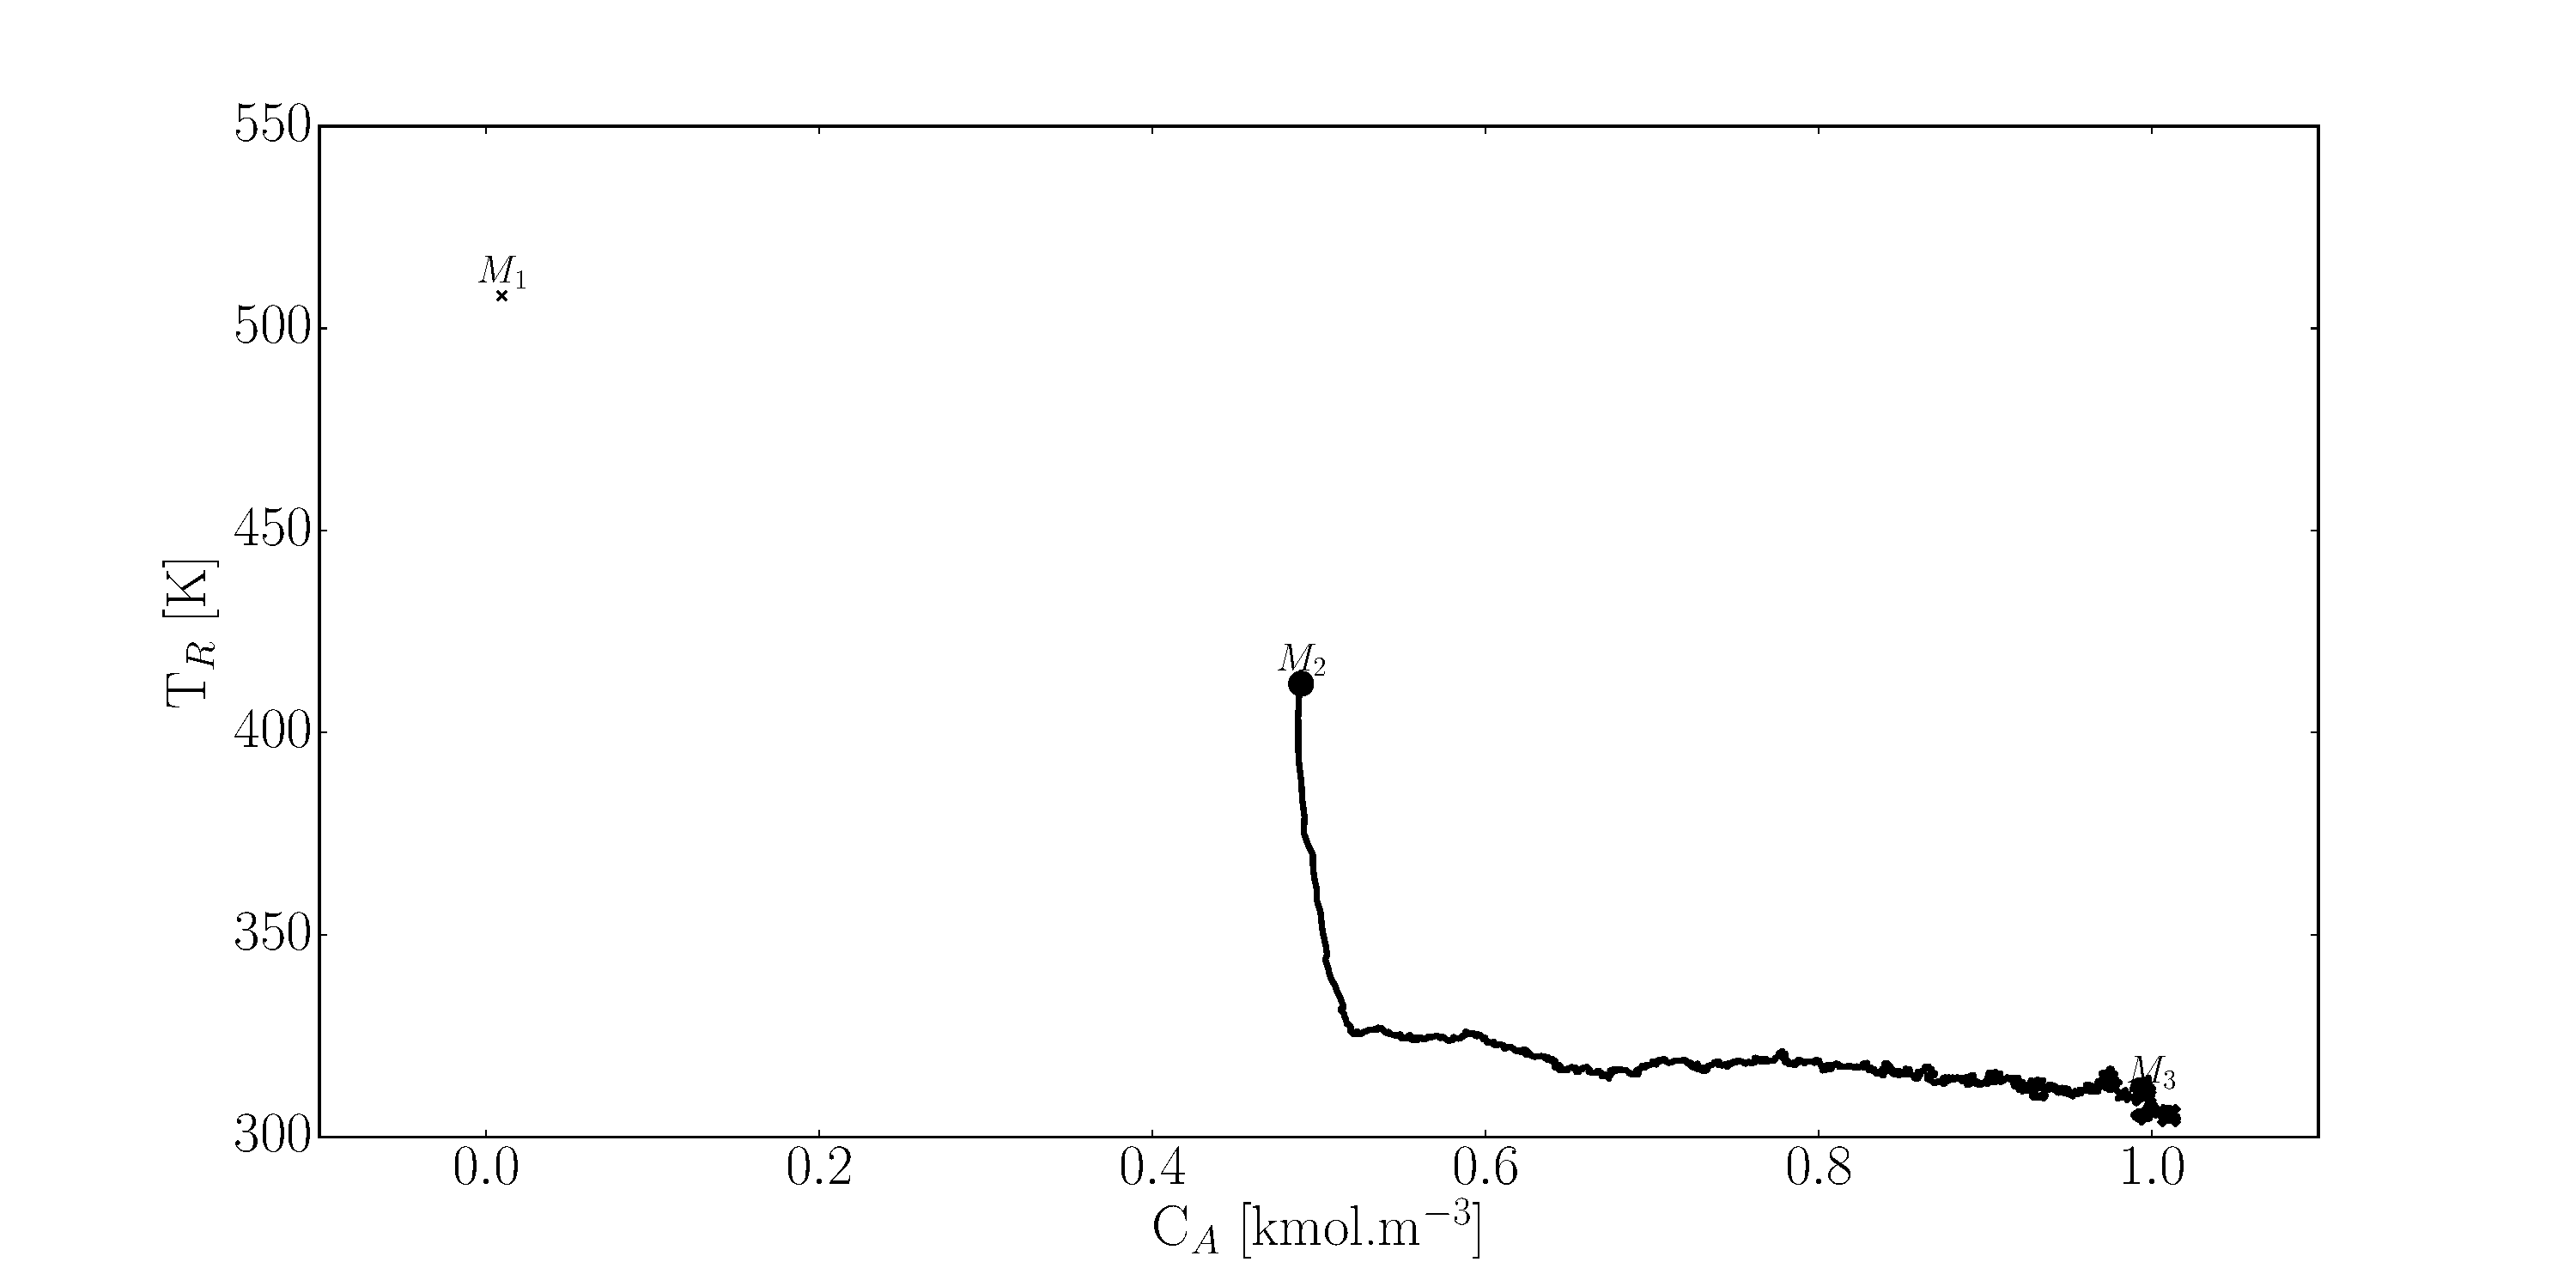
\includegraphics[width=\textwidth]{rbpf_control_state.pdf}
\caption{State space trajectory of the non-linear CSTR under control of the LQG switching controller algorithm. The initial point was $(0.49, 412)$}
\label{fig_rbpf_control_state}
\end{figure}
Figure \ref{fig_rbpf_control_switch} confirms the behaviour we expected: initially $M_2$ best explained the observations but $M_2$ gives way to $M_3$ throughout the rest of the simulation.   
\begin{figure}[H] 
\centering
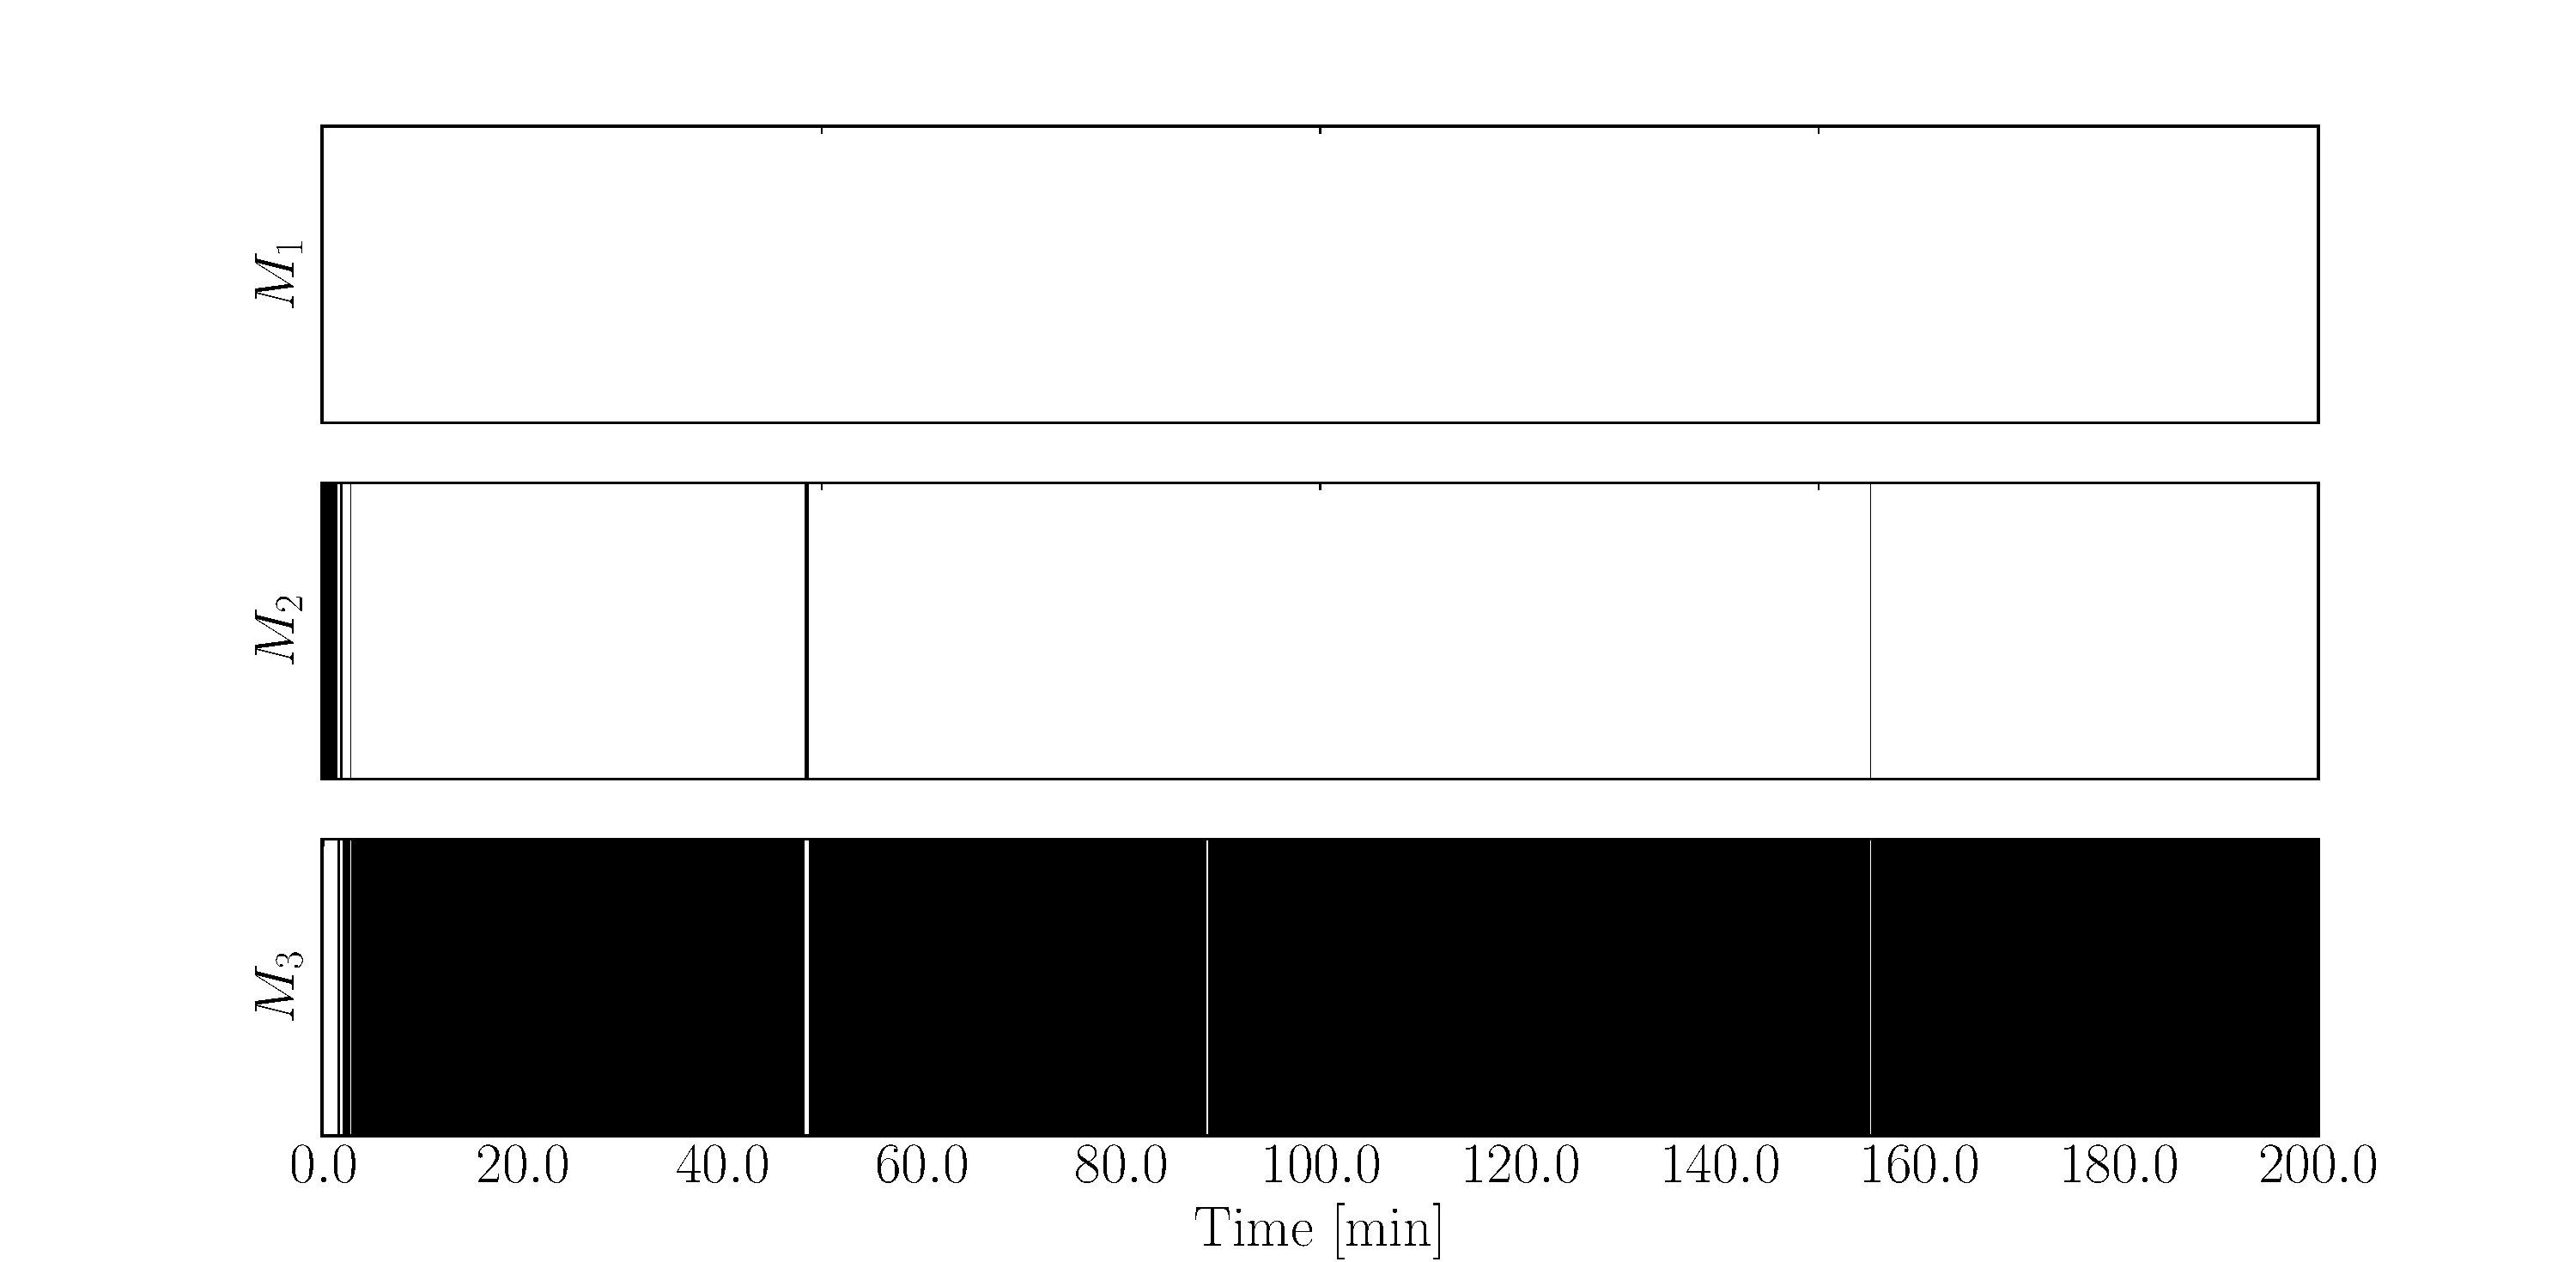
\includegraphics[width=\textwidth]{rbpf_control_switch.pdf}
\caption{Most likely model used for control at each time step over the simulation. Black indicates the model is active.}
\label{fig_rbpf_control_switch}
\end{figure}
However, it is clear that there are some problems in Figure \ref{fig_rbpf_control_switch}. There does seem to be some slight switching noise. Given that we are using the sticky switching transition matrix $P_2$ it is clear that model overlap is causing problems. The same problem was identified in Chapter \ref{sec_rbpf_filtering_cstr}. In Figure \ref{fig_rbpf_control_track} we see the set point tracking performance of the switching controller. It is clear that the controller tracks the set point.
\begin{figure}[H] 
\centering
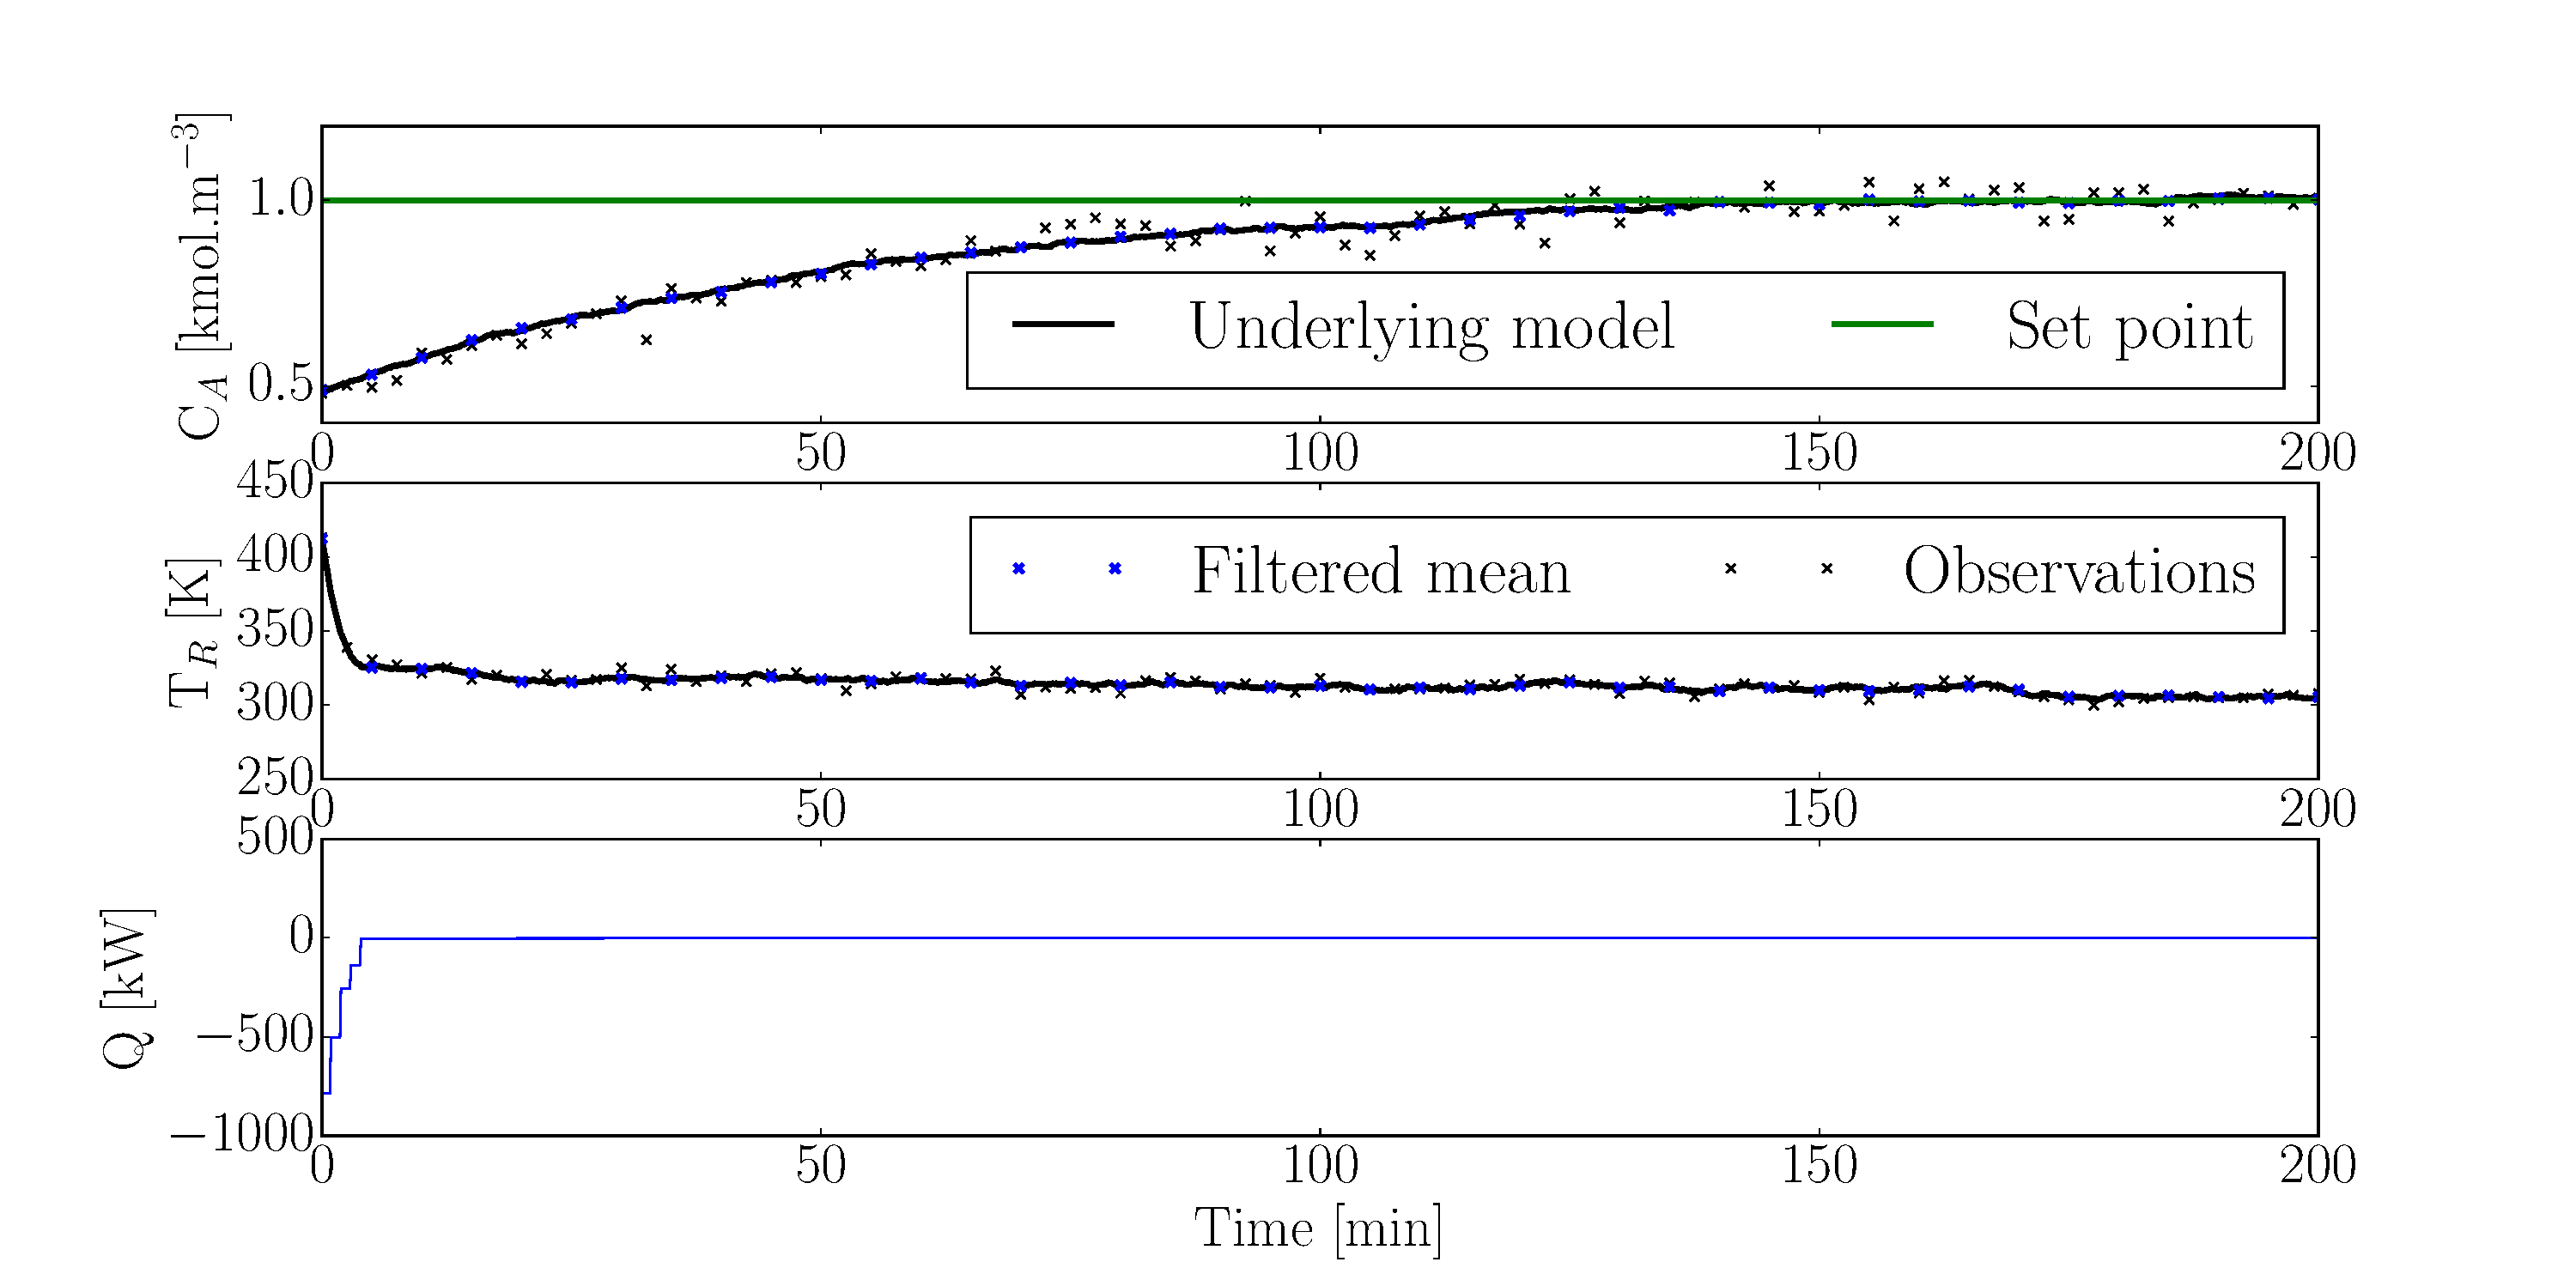
\includegraphics[width=\textwidth]{rbpf_control_track.pdf}
\caption{Set point tracking and controller input for the LQG 3 model switching controller algorithm. The initial point was $(0.49, 412)$.}
\label{fig_rbpf_control_track}
\end{figure}
Based on Figures \ref{fig_rbpf_control_switch} and \ref{fig_rbpf_control_track} it would be too easy to surmise that the controller algorithm works. Unfortunately this is not the case in general. In Figures \ref{fig_rbpf_control_switch2} and \ref{fig_rbpf_control_track2} we study problem 2: tracking the concentration set point of $0.90~\text{kmol.m}^{-3}$. In Figure \ref{fig_rbpf_control_switch2} we see significant model switching noise.
\begin{figure}[H] 
\centering
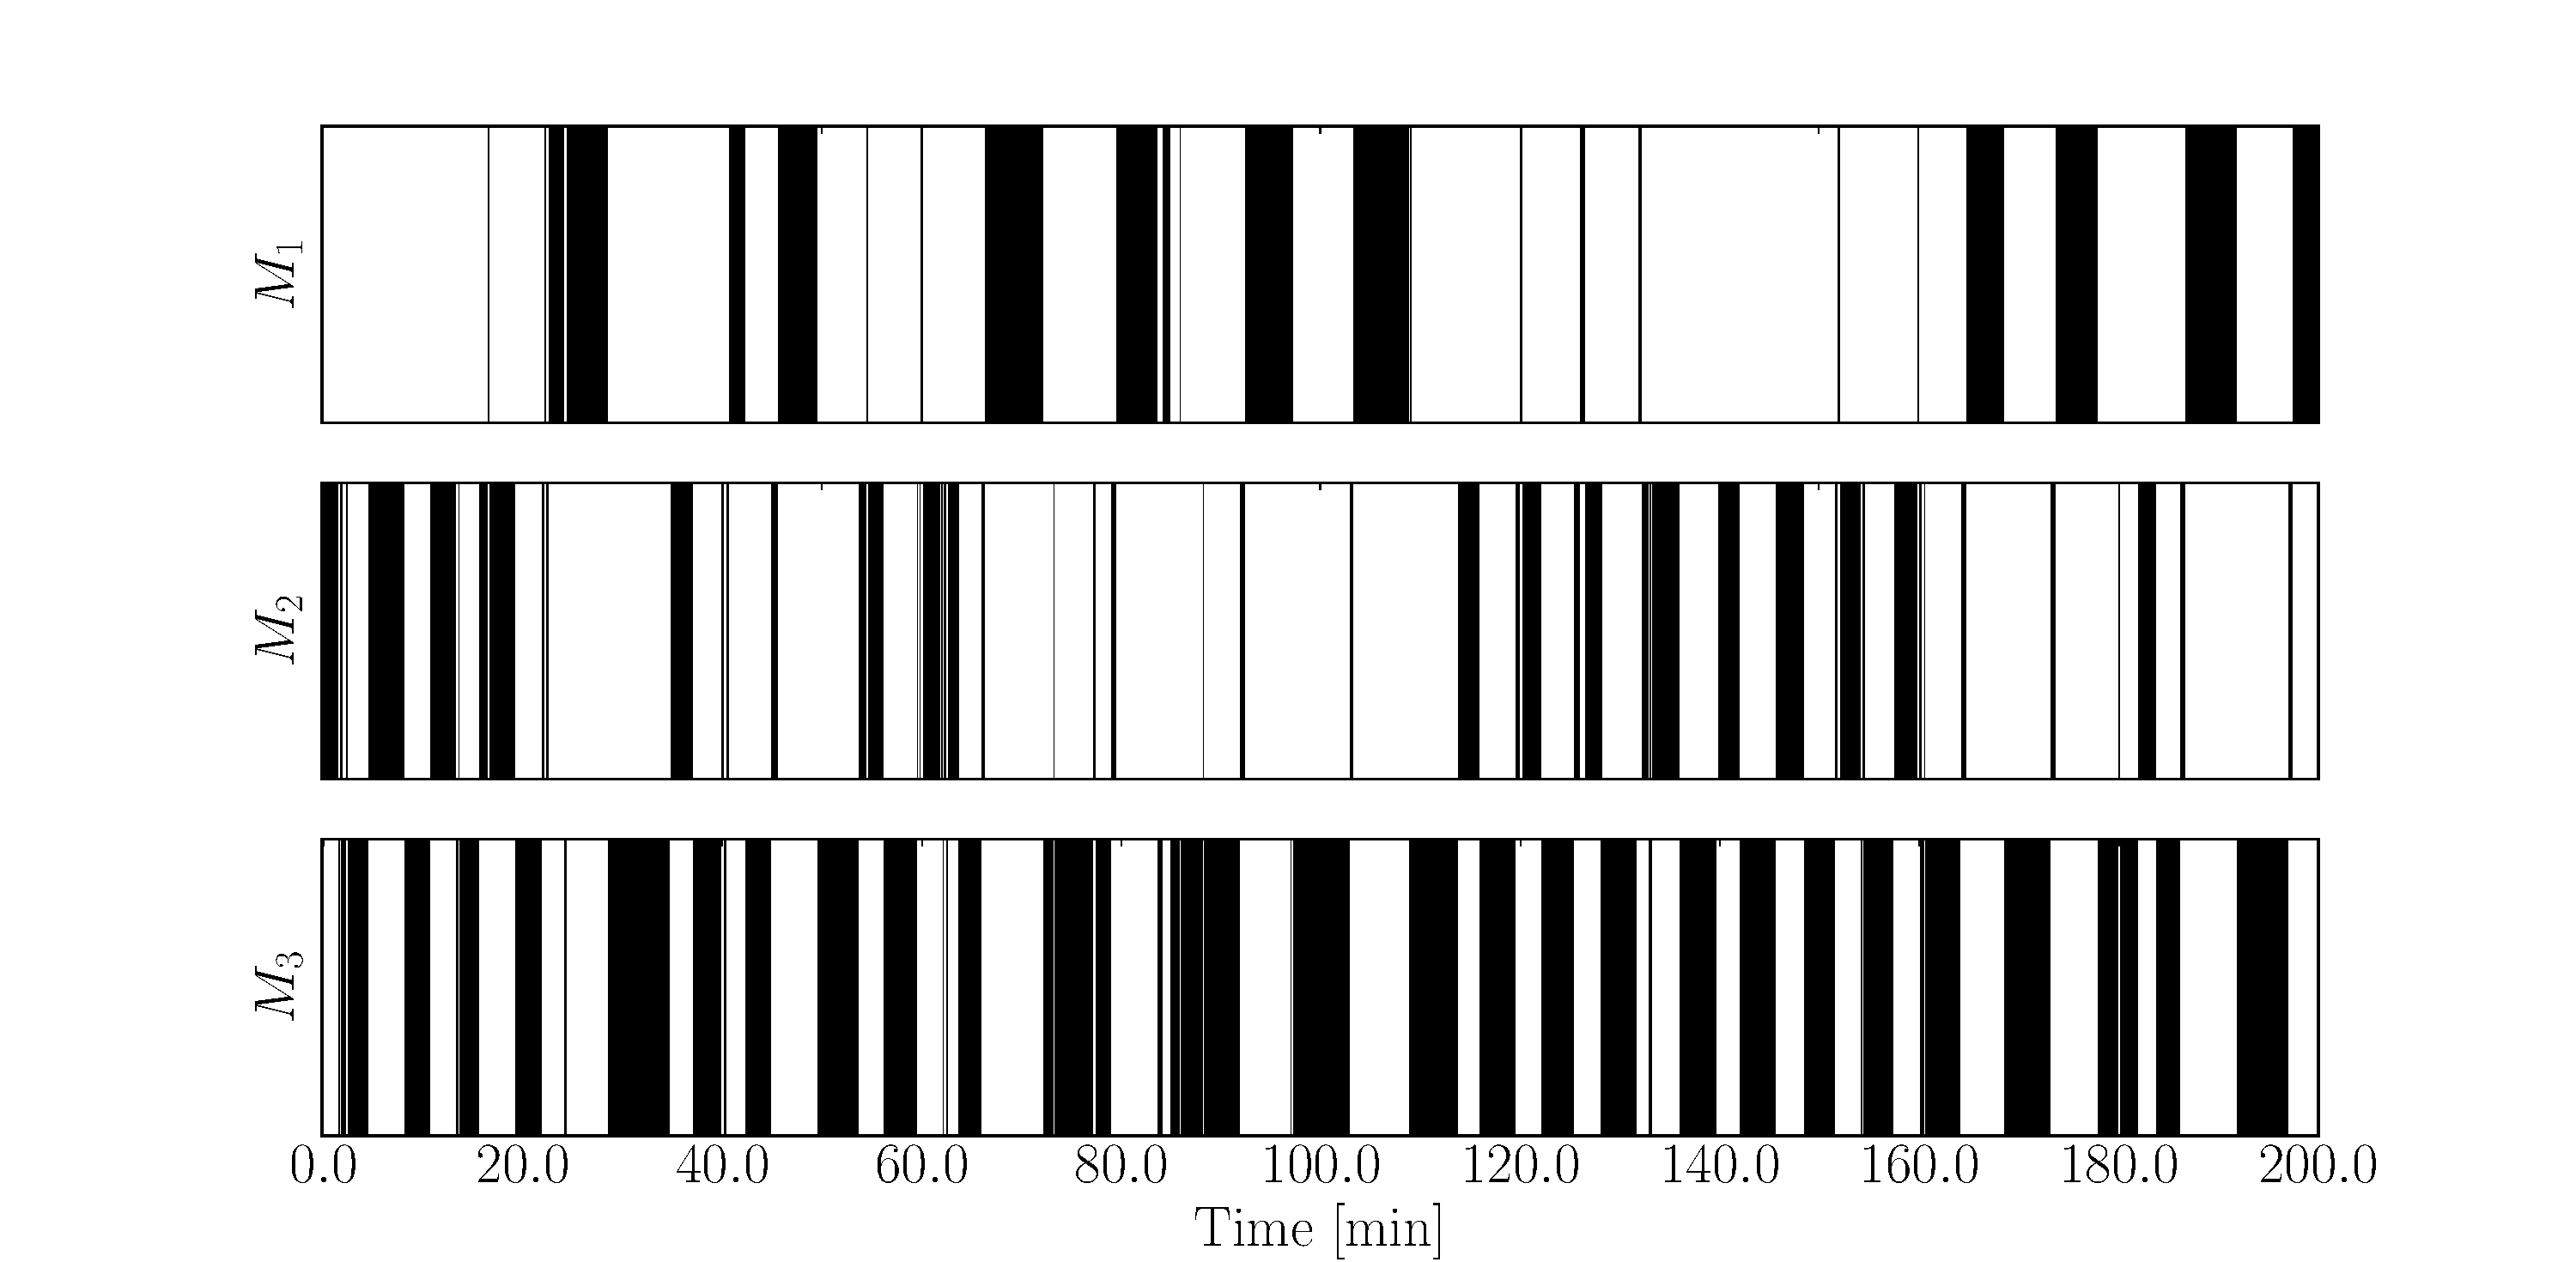
\includegraphics[width=\textwidth]{rbpf_control_switch2.pdf}
\caption{Most likely model used for control at each time step over the simulation. Black indicates the model is active.}
\label{fig_rbpf_control_switch2}
\end{figure}
In Figure \ref{fig_rbpf_control_track2} the detrimental consequence of the switching noise is evident. The controller is completely unstable and oscillates.
\begin{figure}[H] 
\centering
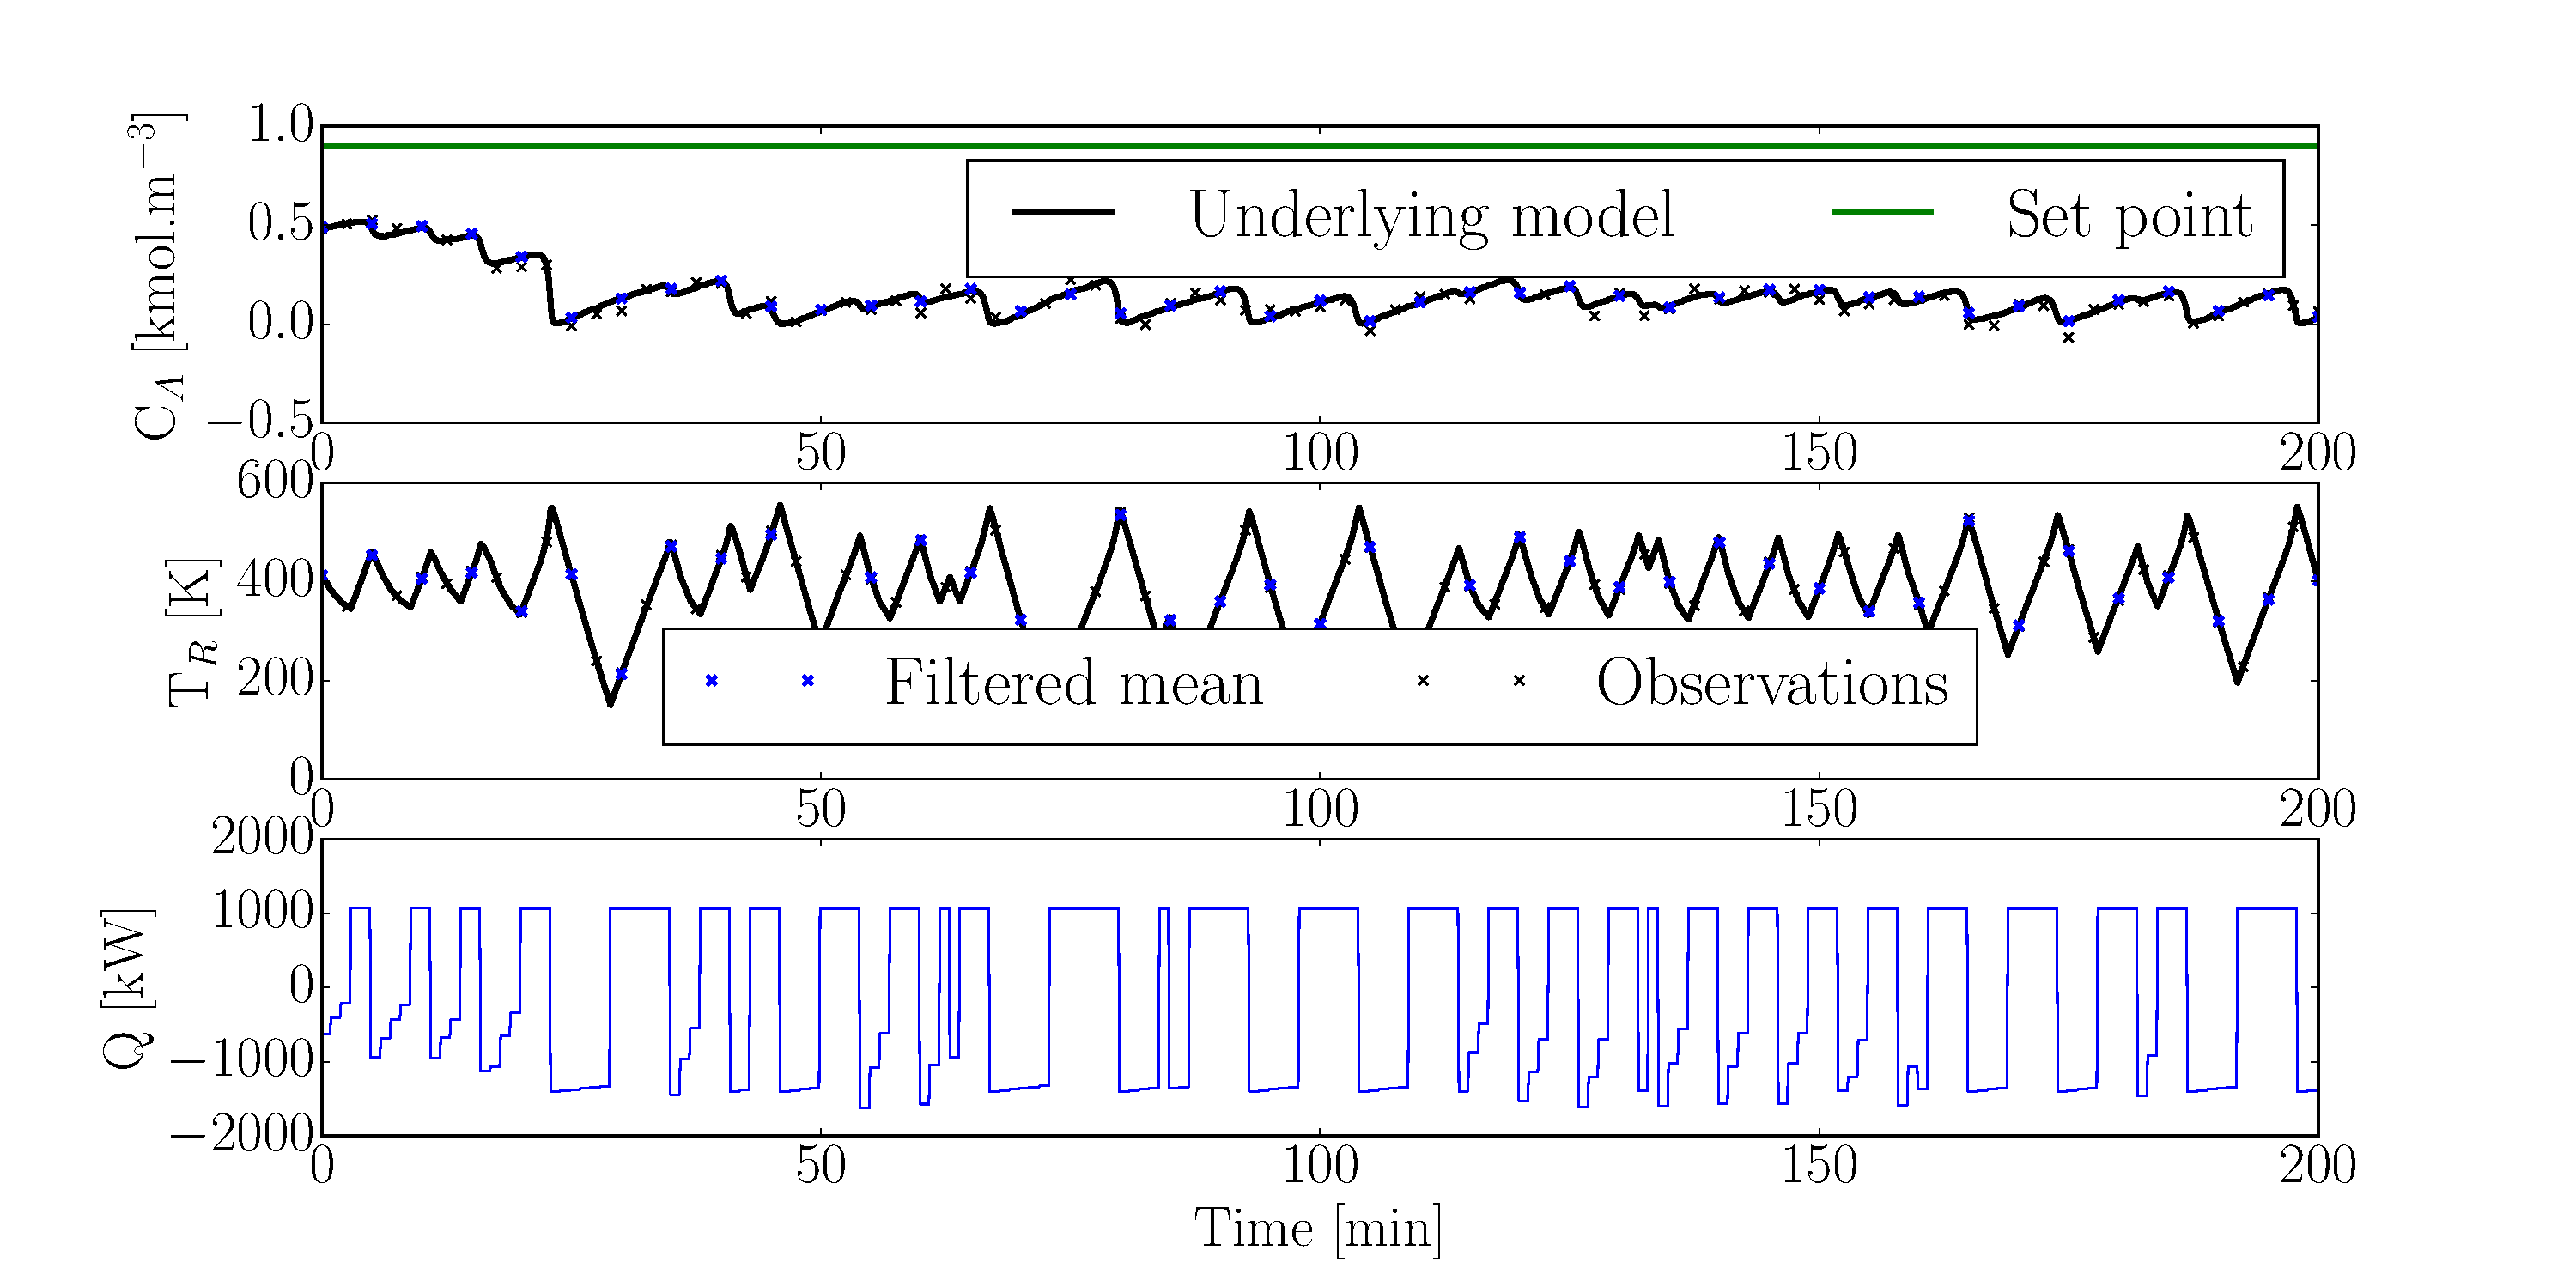
\includegraphics[width=\textwidth]{rbpf_control_track2.pdf}
\caption{Set point tracking and controller input for the LQG 3 model switching controller algorithm. The initial point was $(0.49, 412)$.}
\label{fig_rbpf_control_track2}
\end{figure}
It is clear that the oscillations are caused by the filter's inability to stick to a model. There are two major problems with the switching controller algorithm as adopted in this chapter:
\begin{enumerate}
\item
Fundamentally we are using an inappropriate model for controller prediction during the initial period of the simulation. If we stayed near the current position in state space then the most likely model would predict the future well and thus result in good control. However, we are projecting the controlled states into regions where the current model control is based upon may not a good approximation at all. This is a fundamental problem of our approach - it would be better to incorporate the model switching within the controller prediction (optimisation) process, but this is exactly what we want to avoid due to the computational burden this introduces!
\item
The switching noise is problematic because it can cause the controller to use a model which is good locally but inappropriate with regard to the true underlying position of the system in state space. However, from an inference perspective the noise is not necessarily undesirable. Switching noise can improve the state estimate accuracy - especially in regions between models. It is also important in allowing the filter to switch punctually: making the switching transition matrix too static retards the sensitivity the filter has to model changes.  
\end{enumerate}
We attempt to ameliorate these problems by extending the number of models available to the filter. We use more models to bridge the gap between the current most likely model and where it projects the states during prediction. In Figure \ref{fig_rbpf_control_state3} we illustrate the state space trajectory followed by the system when it has 7 models available for inference and control.
\begin{figure}[H] 
\centering
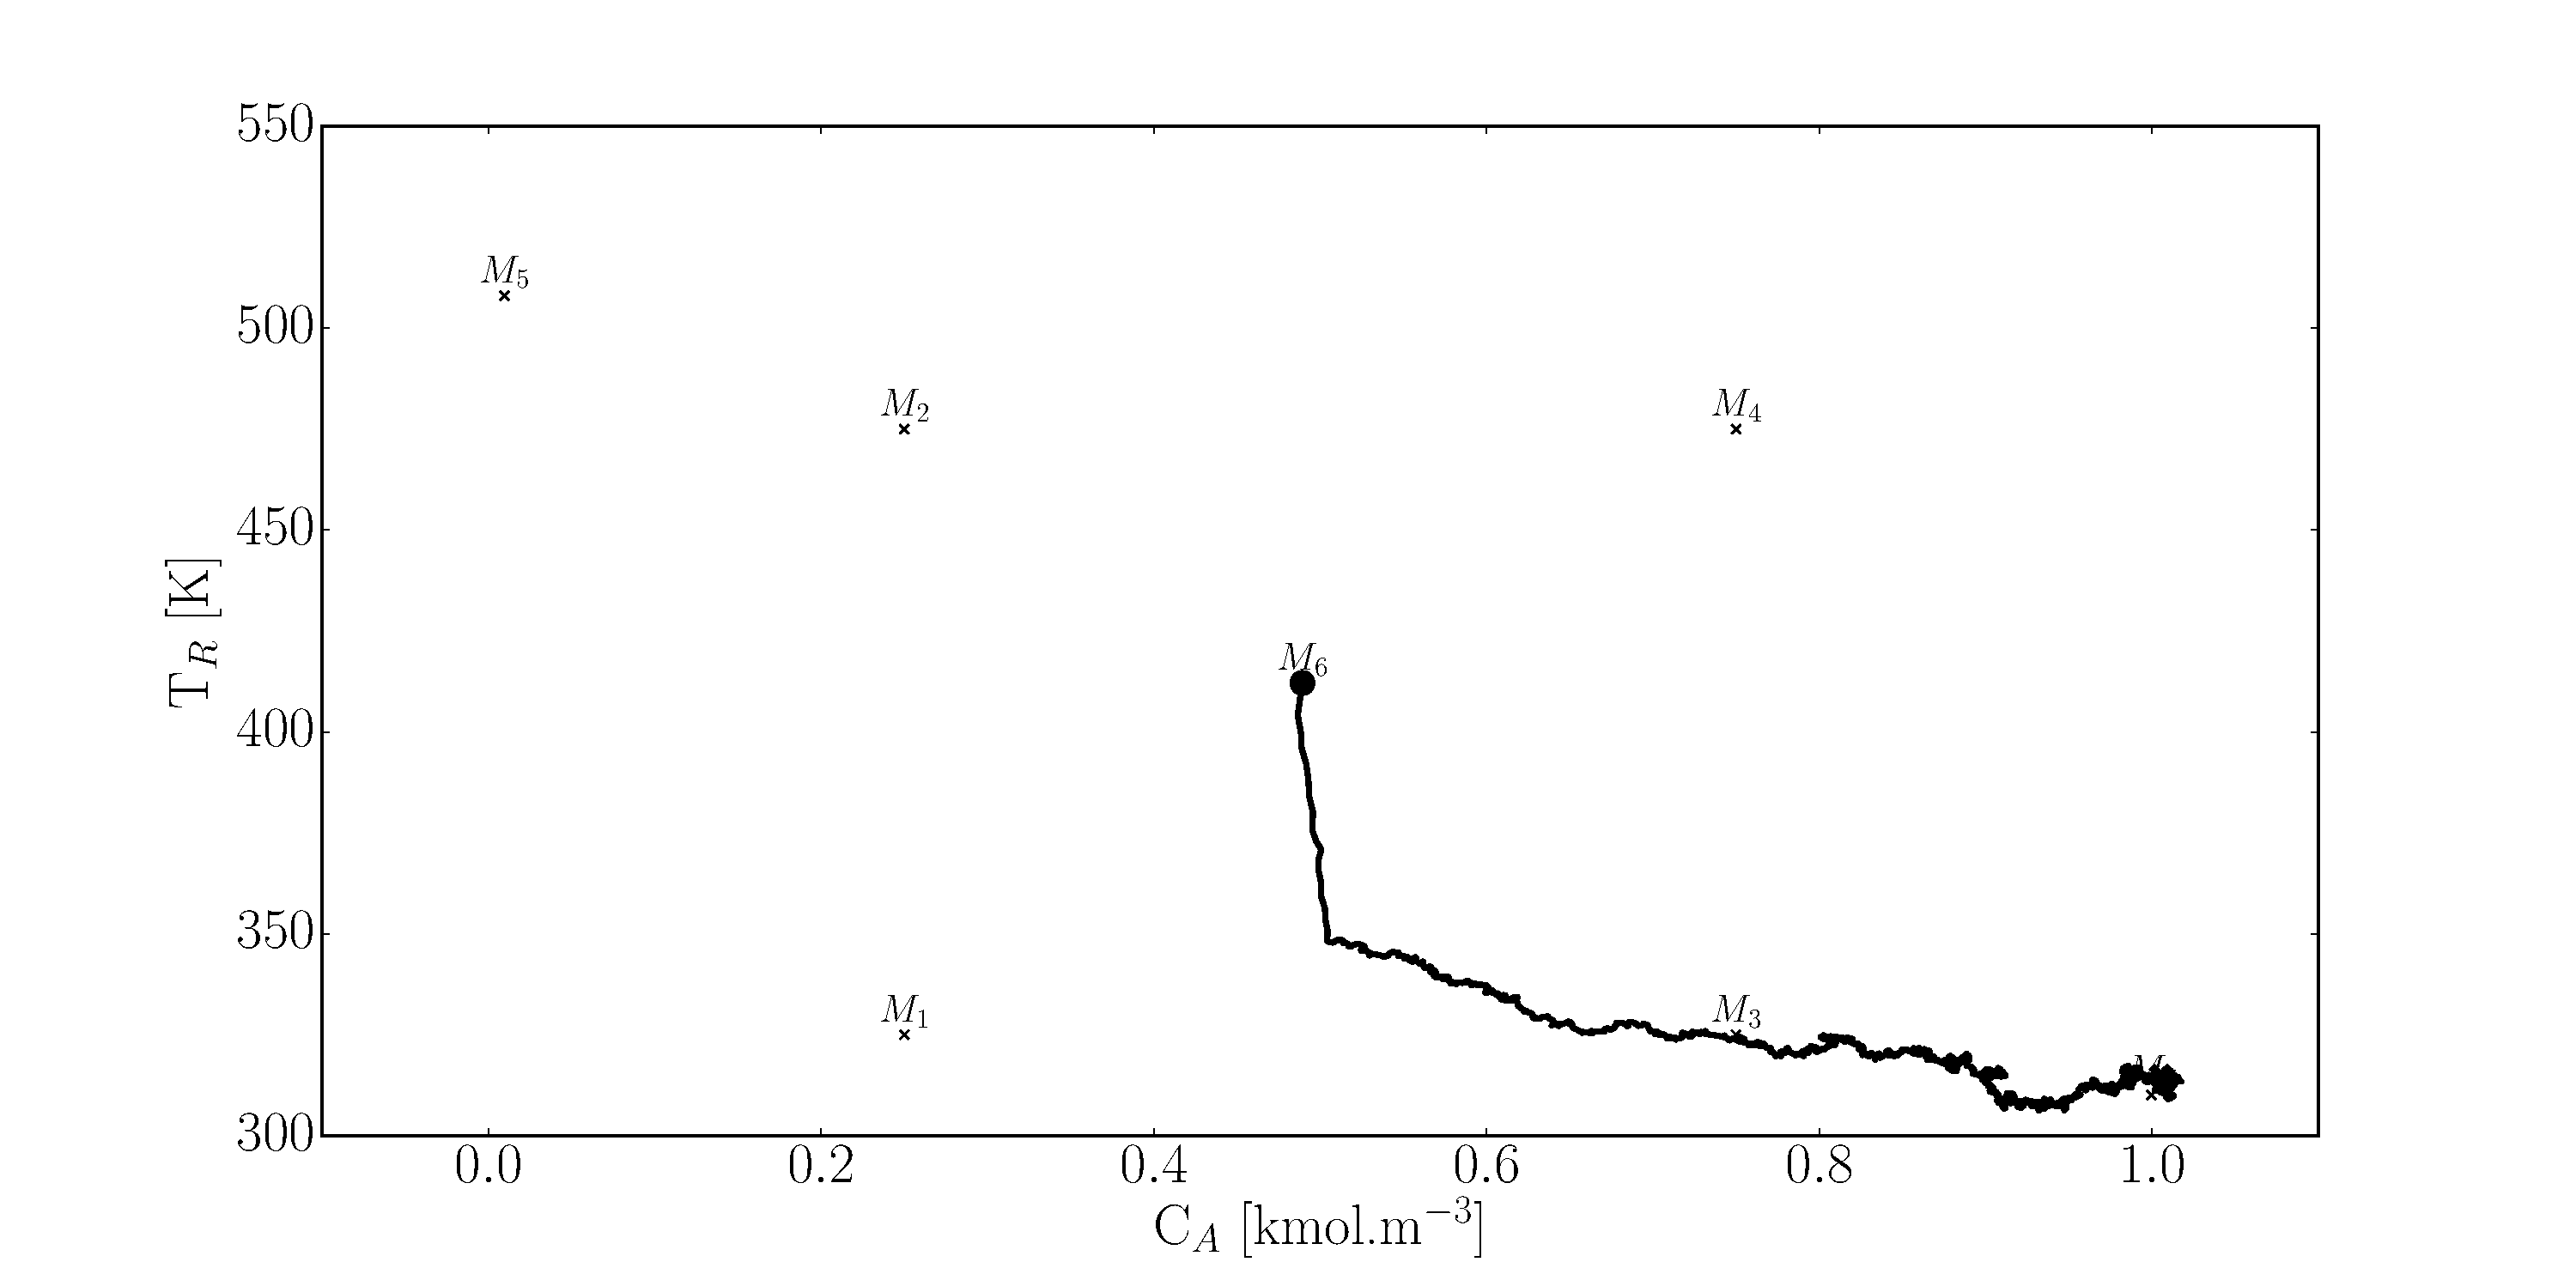
\includegraphics[width=\textwidth]{rbpf_control_state3.pdf}
\caption{State space trajectory of the non-linear CSTR under control of the LQG 7 model switching controller algorithm. The initial point was $(0.49, 412)$}
\label{fig_rbpf_control_state3}
\end{figure}
In Figures \ref{fig_rbpf_control_switch3} and \ref{fig_rbpf_control_track3} we again attempt to steer the system from the unstable operating point to the low temperature operating point. Figure \ref{fig_rbpf_control_switch3} shows which models were active over the simulation window.
\begin{figure}[H] 
\centering
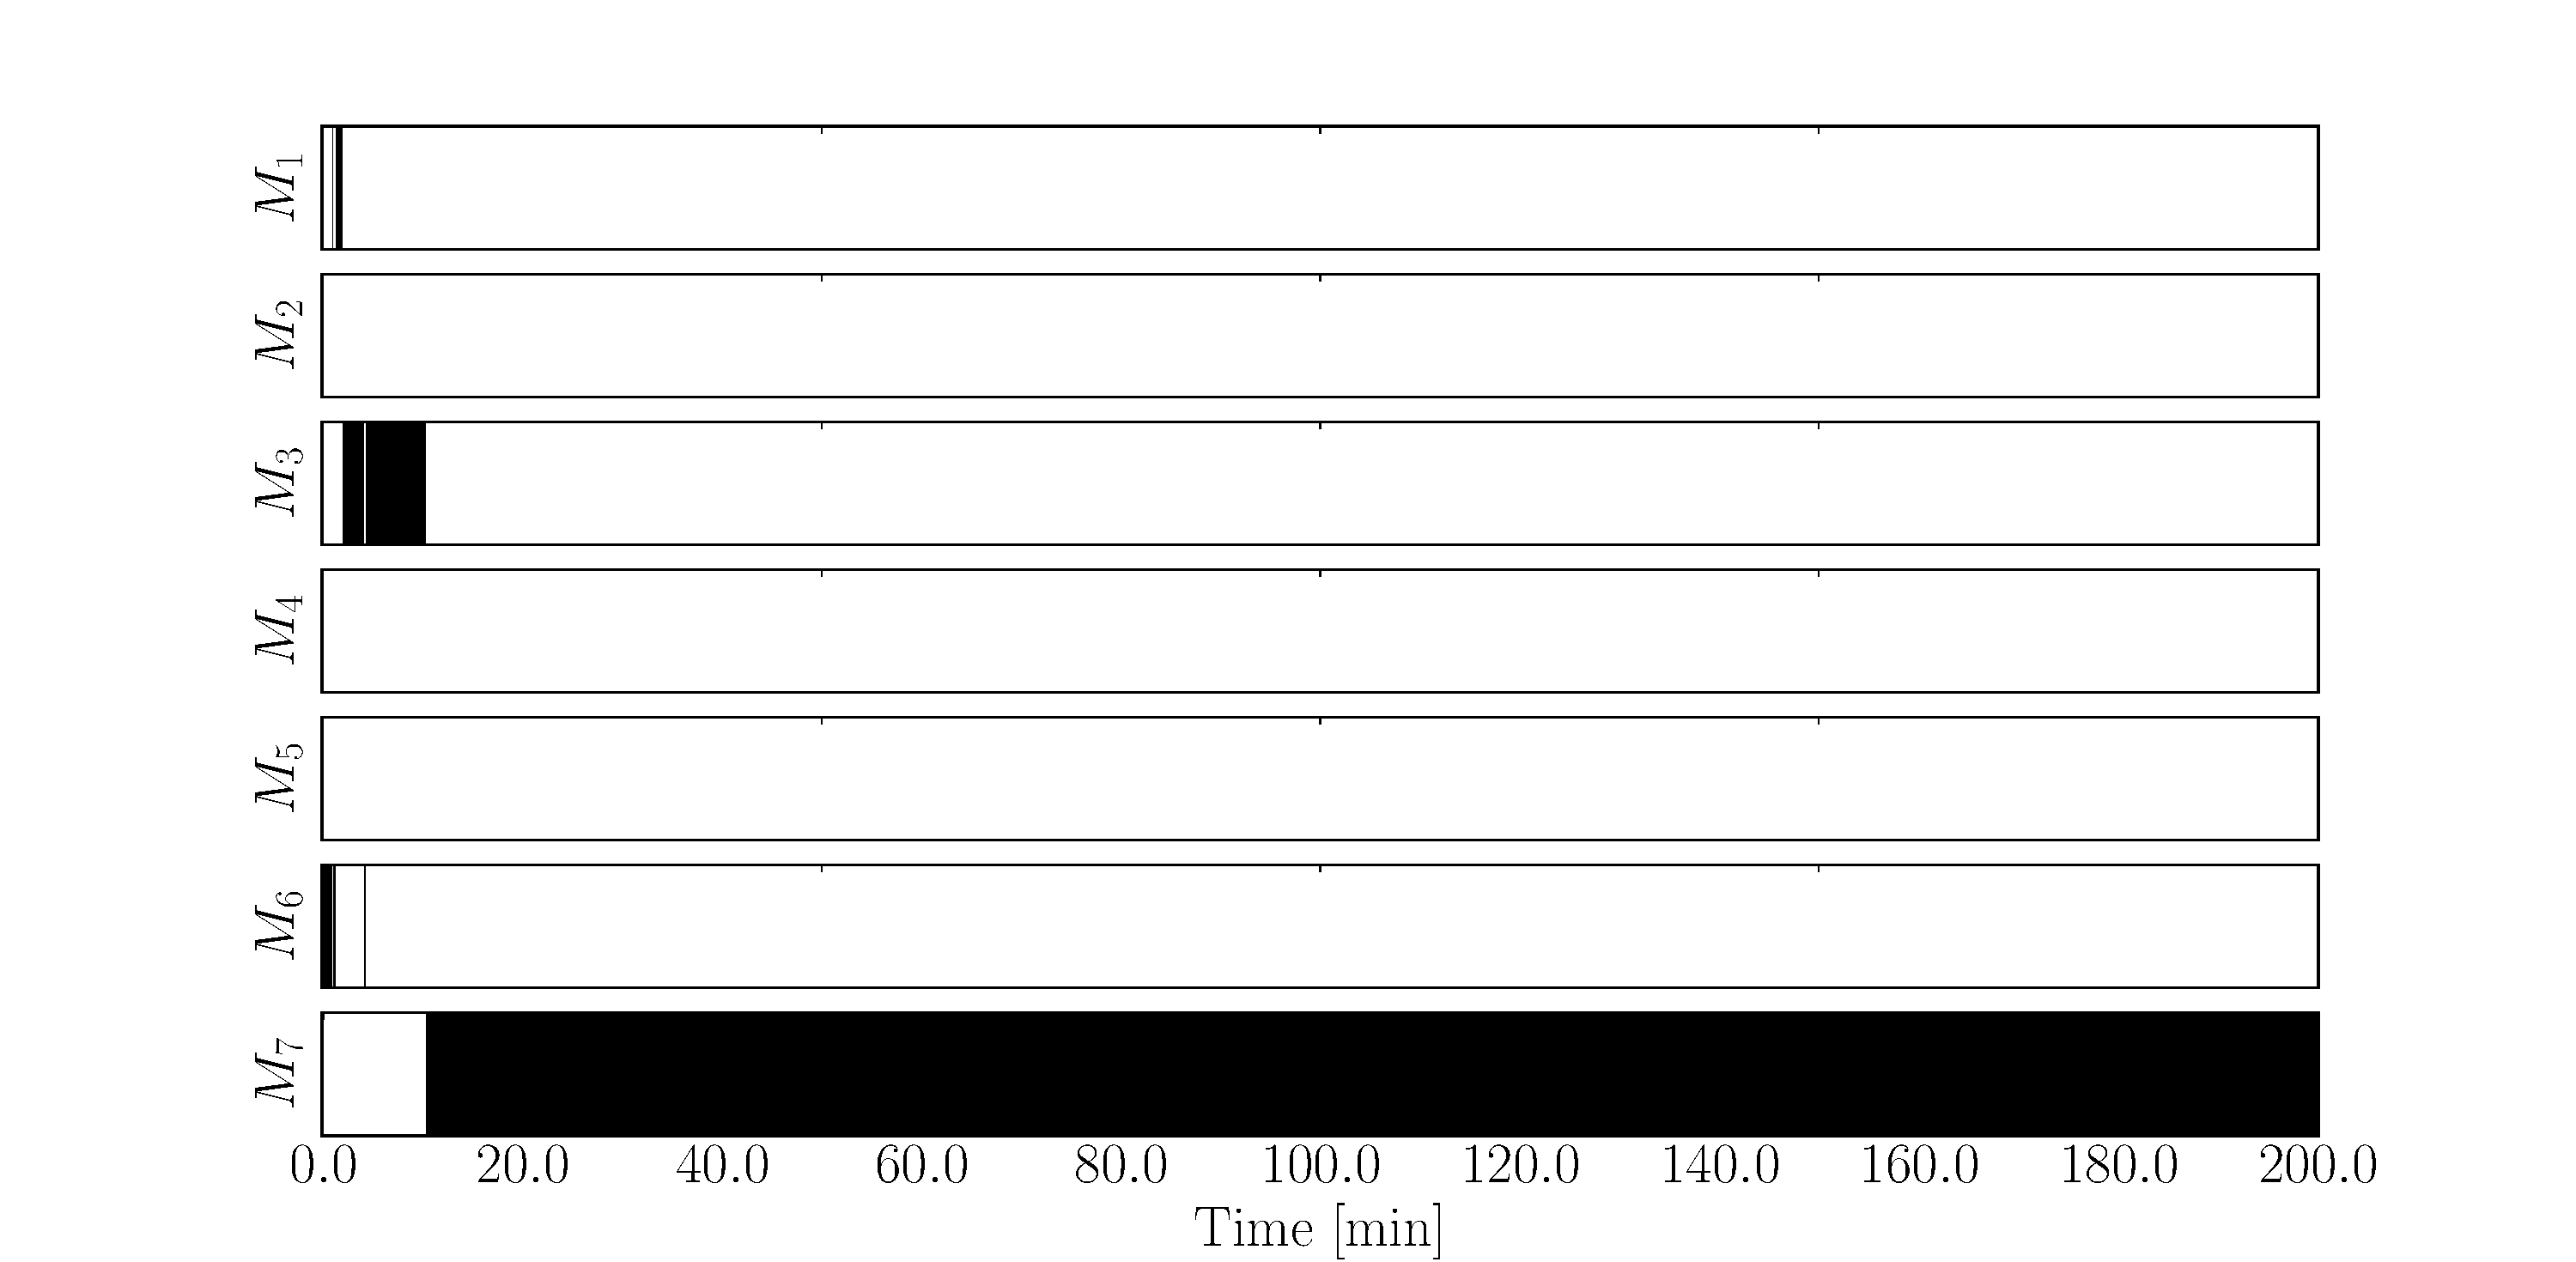
\includegraphics[width=\textwidth]{rbpf_control_switch3.pdf}
\caption{Most likely model used for control at each time step over the simulation. Black indicates the model is active.}
\label{fig_rbpf_control_switch3}
\end{figure}
While there is slight switching noise the model selection is exactly what one would expect. Figure \ref{fig_rbpf_control_track3} shows the controller set point tracking performance over the simulation window.
\begin{figure}[H] 
\centering
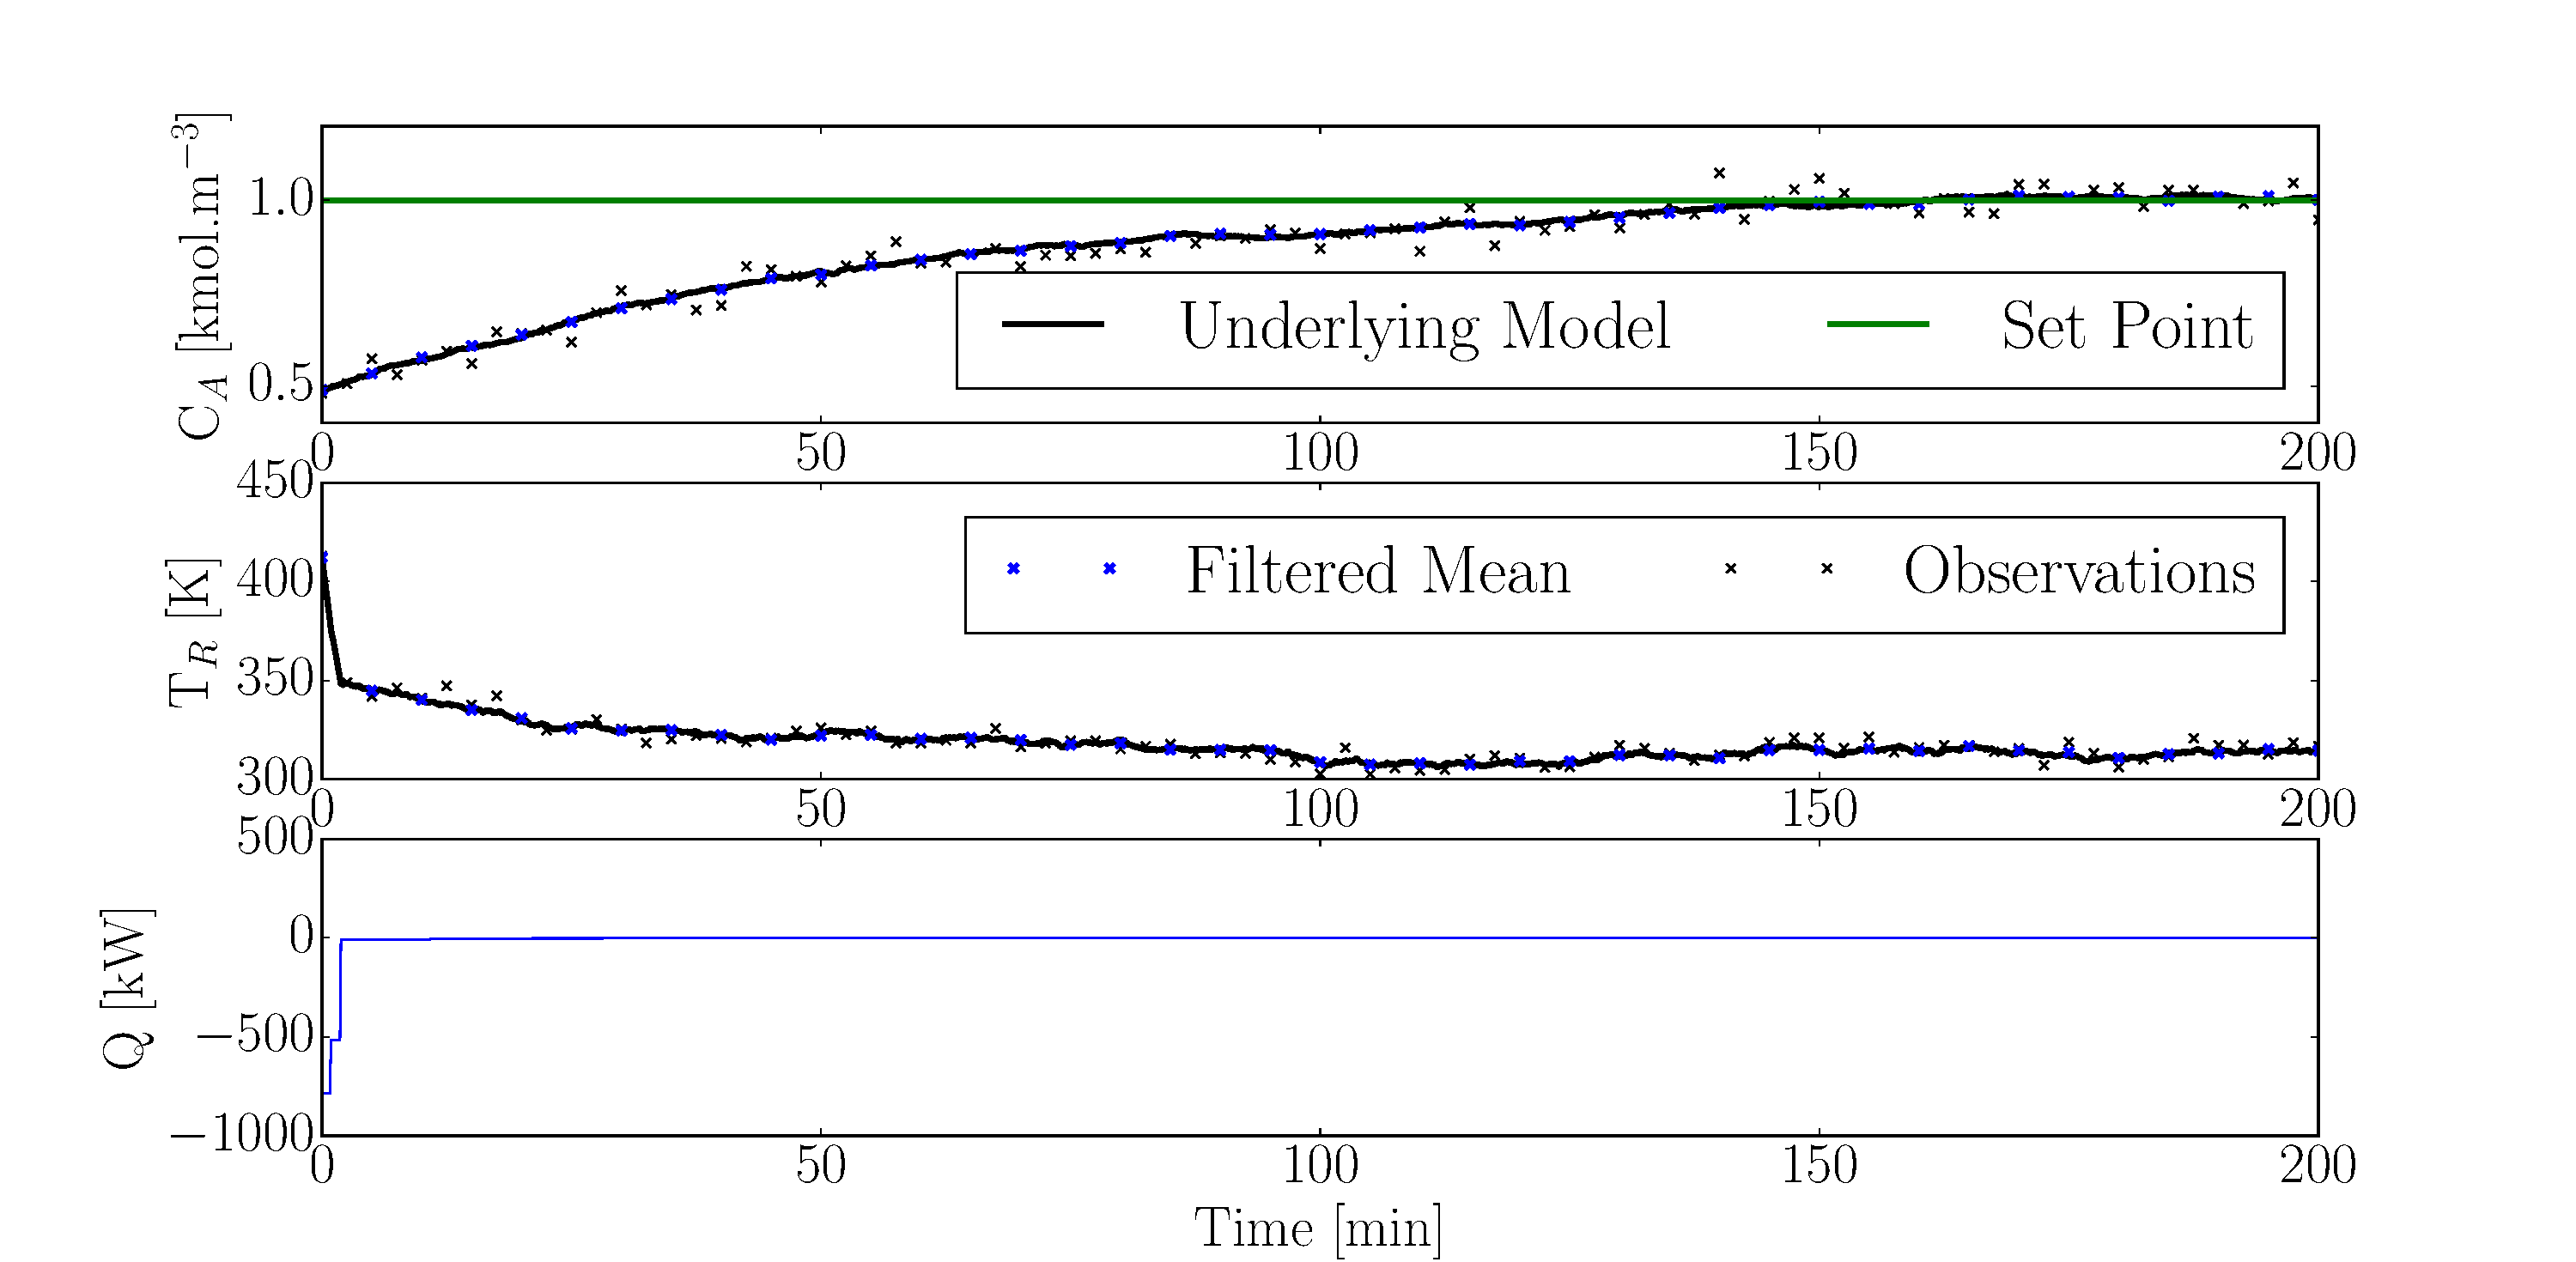
\includegraphics[width=\textwidth]{rbpf_control_track3.pdf}
\caption{Set point tracking and controller input for the LQG 7 model switching controller algorithm. The initial point was $(0.49, 412)$.}
\label{fig_rbpf_control_track3}
\end{figure}
Like Figure \ref{fig_rbpf_control_track} we also have a stable, reference tracking controller. This is not surprising because the model switching/selection was reasonable. In Figure \ref{fig_rbpf_control_switch4} and \ref{fig_rbpf_control_track4} we again attempt to steer the system to a concentration set point of $0.9$ kmol.m$^{-3}$. Since we introduced $M_3$ to serve as a bridge between $M_6$ and $M_7$ (since the set point is between these two models) we expect better performance than in Figure \ref{fig_rbpf_control_switch2} and \ref{fig_rbpf_control_track2}. Unfortunately this is not the case as may be seen in Figures \ref{fig_rbpf_control_switch4} and \ref{fig_rbpf_control_track4}.
\begin{figure}[H] 
\centering
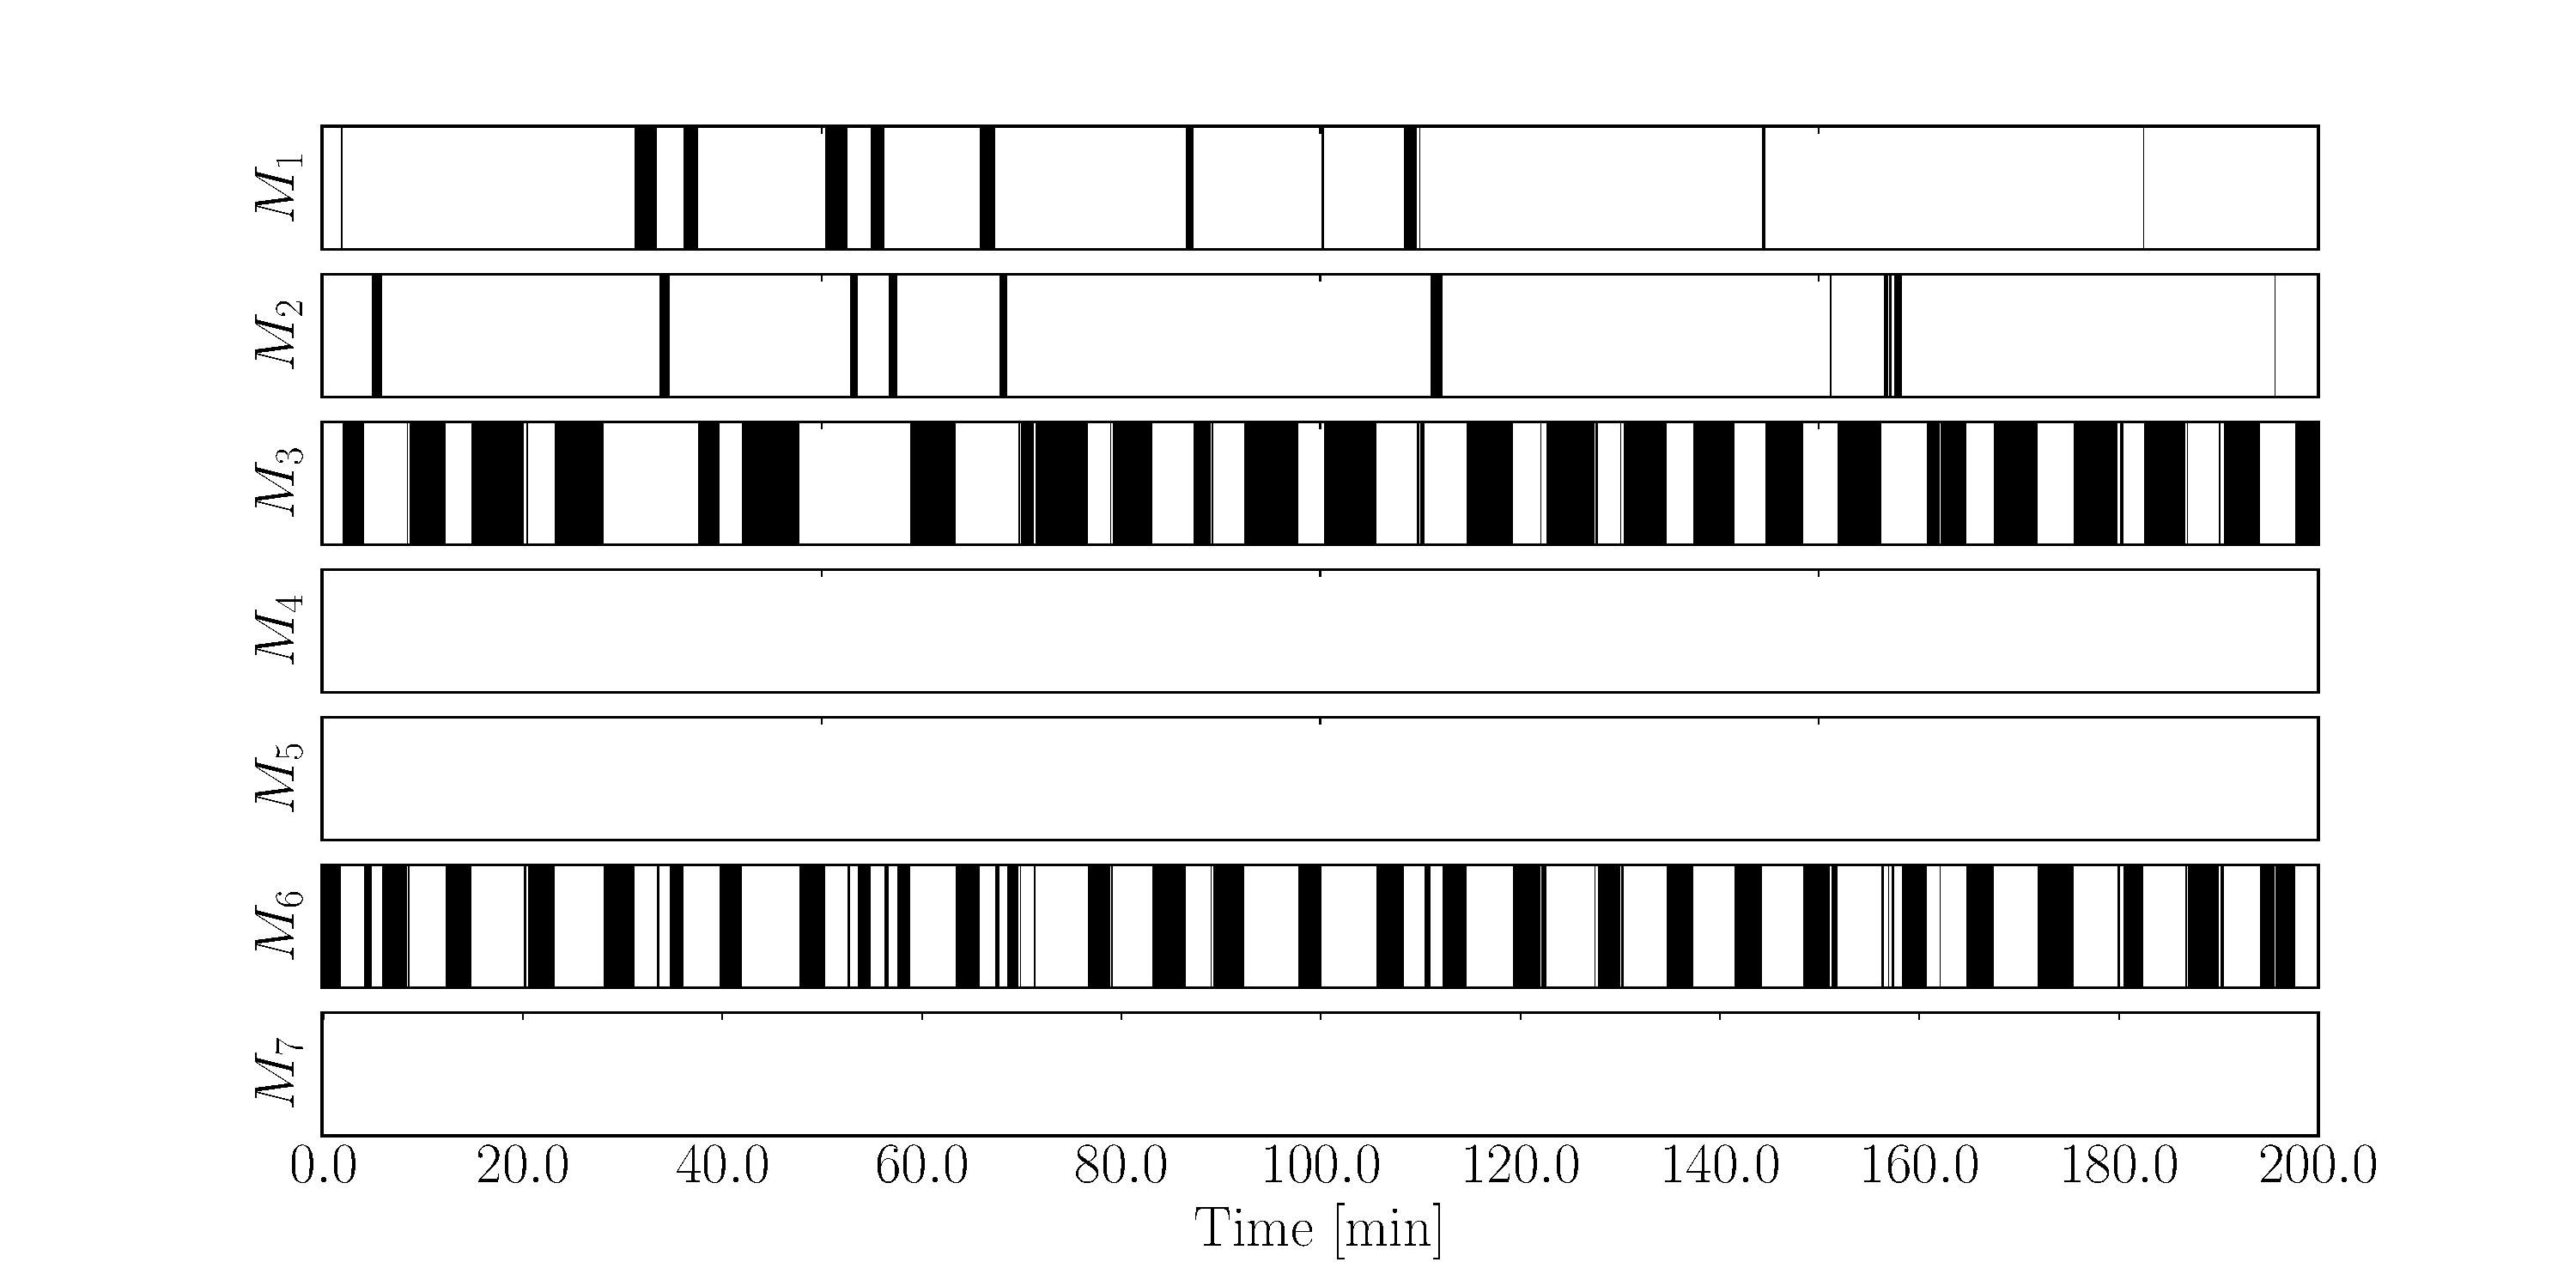
\includegraphics[width=\textwidth]{rbpf_control_switch4.pdf}
\caption{Most likely model used for control at each time step over the simulation. Black indicates the model is active.}
\label{fig_rbpf_control_switch4}
\end{figure}
The same oscillating switching noise and unstable control is present here as there was in Figures \ref{fig_rbpf_control_switch2} and \ref{fig_rbpf_control_track2}.
\begin{figure}[H] 
\centering
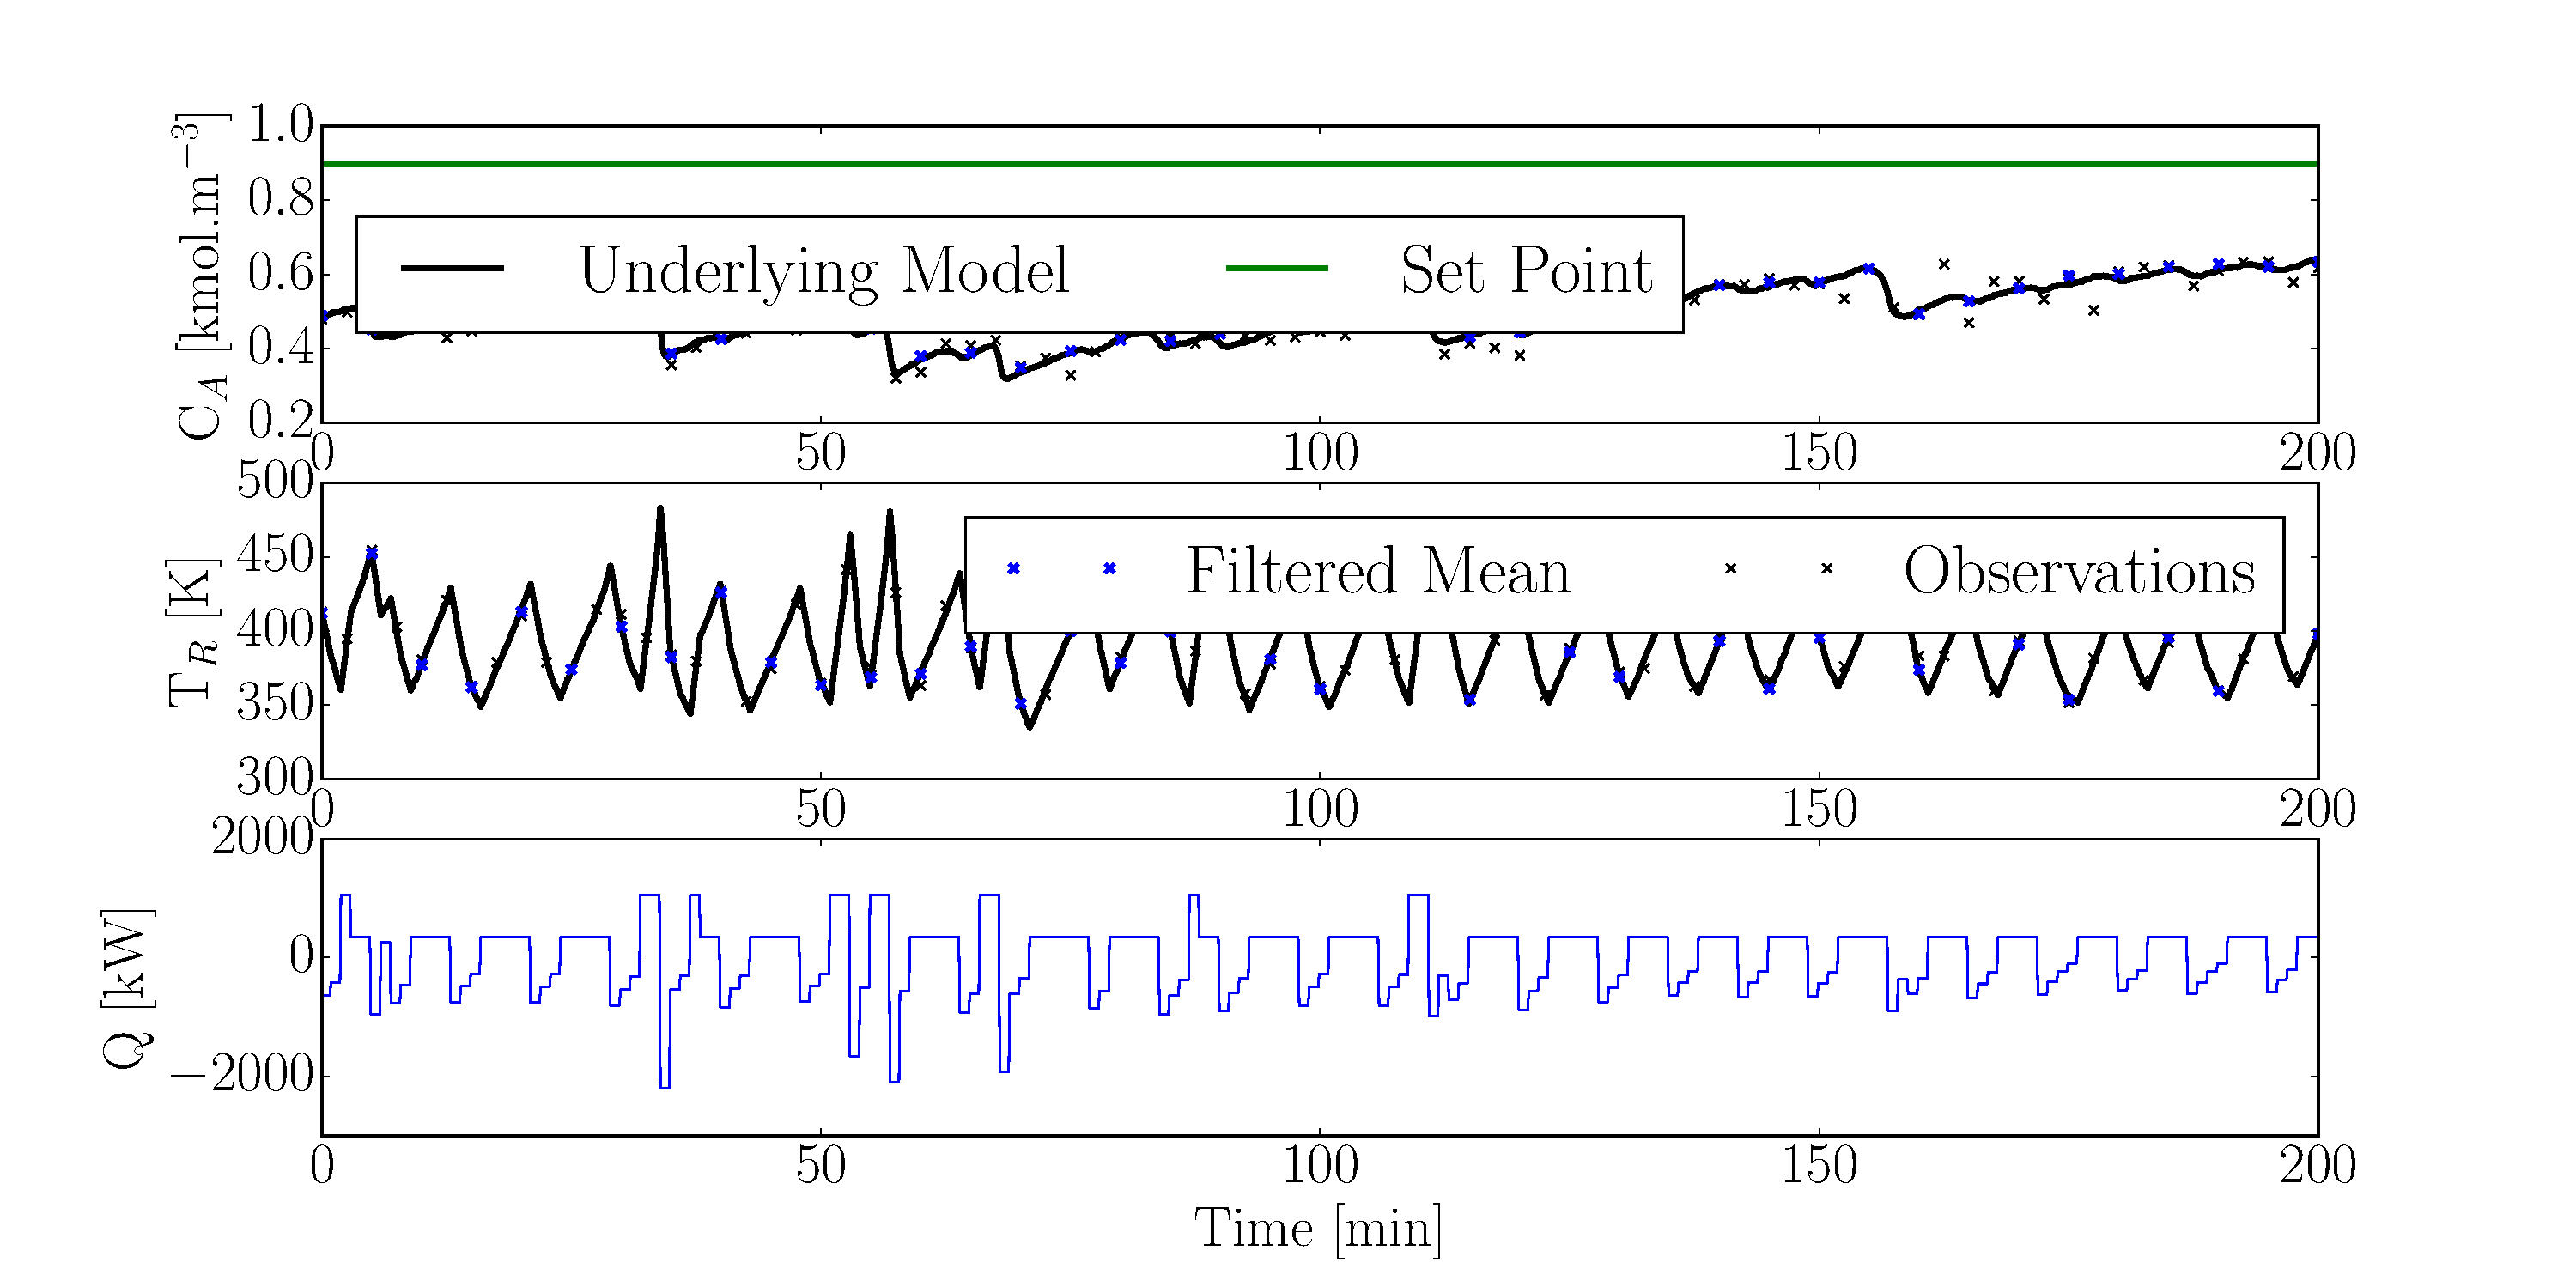
\includegraphics[width=\textwidth]{rbpf_control_track4.pdf}
\caption{Set point tracking and controller input for the LQG 7 model switching controller algorithm. The initial point was $(0.49, 412)$.}
\label{fig_rbpf_control_track4}
\end{figure}
The underlying reasons for the instability are the same: we are using models to predict into regions where they are inaccurate and the filter does not robustly enough isolate the model closest to the current system location in state space. The combination of these two problems make effective control impossible.

\subsection{Model averaging approach}
\label{sec_ma_rbpf}
The fundamental problem with the switching controllers of Chapter \ref{sec_rbpf_control_uncon} is that an inappropriate model was used for prediction. Unfortunately using a weighted average of all the models, based on their probability with respect to the switching variable $s_t$, will exacerbate this problem. For this reason we do not explore this approach.

\section{Conclusion}
The goal of the switching controller algorithm was to drastically reduce the computational burden introduced by modern switching controller implementations as discussed in Chapter \ref{sec_switch_mpc_lit}. The approach of switching the model used for control outside the optimisation algorithm, while attractive intuitively, suffers from the fundamental problem that a bad model is used to predict the future states.

The switching LQG controllers introduced in this chapter were not robust against this type of problem. Additionally, we also had severe switching noise which led to controller oscillation. From a fundamental point of view it seems as if the current approach of incorporating the model switching inside the optimisation algorithm has the most promise of yielding good control. 

It should be investigated whether it is feasible to incorporate the Rao-Blackwellised particle prediction (see Chapter \ref{sec_inf_rbpf_pred}) within the controller optimisation process.  